
\documentclass[working]{tuftebook}

\usepackage[utf8]{inputenc}
\usepackage[T1]{fontenc}
\usepackage{textcomp}

\usepackage{url}

\usepackage[
    sorting=nyt,
    style=alphabetic
]{biblatex}
\addbibresource{bibliography.bib}

\usepackage{hyperref}
\hypersetup{
    colorlinks,
    linkcolor={black},
    citecolor={black},
    urlcolor={blue!80!black}
}
\usepackage[noabbrev]{cleveref}

% Adds Bibliography, ... to Table of Contents
\usepackage[nottoc]{tocbibind}

\usepackage{graphicx}
\usepackage{float}
\usepackage[usenames,dvipsnames,svgnames]{xcolor}

% \usepackage{cmbright}

\usepackage{amsmath, amsfonts, mathtools, amsthm, amssymb}
\usepackage{mathrsfs}
\usepackage{cancel}

\newcommand\N{\ensuremath{\mathbb{N}}}
\newcommand\R{\ensuremath{\mathbb{R}}}
\newcommand\Z{\ensuremath{\mathbb{Z}}}
\renewcommand\O{\ensuremath{\emptyset}}
\newcommand\Q{\ensuremath{\mathbb{Q}}}
\newcommand\C{\ensuremath{\mathbb{C}}}
\let\implies\Rightarrow
\let\impliedby\Leftarrow
\let\iff\Leftrightarrow
\let\epsilon\varepsilon

\usepackage{tikz}
\usepackage{tikz-cd}

% theorems
\usepackage{thmtools}
\usepackage{thm-restate}
\usepackage[framemethod=TikZ]{mdframed}
\mdfsetup{skipabove=1em,skipbelow=0em, innertopmargin=12pt, innerbottommargin=8pt}

\theoremstyle{definition}

\makeatletter

\declaretheoremstyle[headfont=\bfseries\sffamily, bodyfont=\normalfont, mdframed={ nobreak } ]{thmgreenbox}
\declaretheoremstyle[headfont=\bfseries\sffamily, bodyfont=\normalfont, mdframed={ nobreak } ]{thmredbox}
\declaretheoremstyle[headfont=\bfseries\sffamily, bodyfont=\normalfont]{thmbluebox}
\declaretheoremstyle[headfont=\bfseries\sffamily, bodyfont=\normalfont]{thmblueline}
\declaretheoremstyle[headfont=\bfseries\sffamily, bodyfont=\normalfont, numbered=no, mdframed={ rightline=false, topline=false, bottomline=false, }, qed=\qedsymbol ]{thmproofbox}
\declaretheoremstyle[headfont=\bfseries\sffamily, bodyfont=\normalfont, numbered=no, mdframed={ nobreak, rightline=false, topline=false, bottomline=false } ]{thmexplanationbox}

\declaretheoremstyle[headfont=\bfseries\sffamily, bodyfont=\normalfont, numbered=no, mdframed={ nobreak, rightline=false, topline=false, bottomline=false } ]{thmexplanationbox}


\declaretheorem[numberwithin=chapter, style=thmgreenbox, name=Definition]{definition}
\declaretheorem[sibling=definition, style=thmredbox, name=Corollary]{corollary}
\declaretheorem[sibling=definition, style=thmredbox, name=Proposition]{prop}
\declaretheorem[sibling=definition, style=thmredbox, name=Theorem]{theorem}
\declaretheorem[sibling=definition, style=thmredbox, name=Lemma]{lemma}
\declaretheorem[sibling=definition, style=thmbluebox,  name=Example]{eg}
\declaretheorem[sibling=definition, style=thmbluebox,  name=Nonexample]{noneg}
\declaretheorem[sibling=definition, style=thmblueline, name=Remark]{remark}




\declaretheorem[numbered=no, style=thmexplanationbox, name=Proof]{explanation}
\declaretheorem[numbered=no, style=thmproofbox, name=Proof]{replacementproof}
\declaretheorem[style=thmbluebox,  numbered=no, name=Exercise]{ex}
\declaretheorem[style=thmblueline, numbered=no, name=Note]{note}

% \renewenvironment{proof}[1][\proofname]{\begin{replacementproof}}{\end{replacementproof}}

% \AtEndEnvironment{eg}{\null\hfill$\diamond$}%

\newtheorem*{uovt}{UOVT}
\newtheorem*{notation}{Notation}
\newtheorem*{previouslyseen}{As previously seen}
\newtheorem*{problem}{Problem}
\newtheorem*{observe}{Observe}
\newtheorem*{property}{Property}
\newtheorem*{intuition}{Intuition}


\declaretheoremstyle[
    headfont=\bfseries\sffamily\color{RawSienna!70!black}, bodyfont=\normalfont,
    mdframed={
        linewidth=2pt,
        rightline=false, topline=false, bottomline=false,
        linecolor=RawSienna, backgroundcolor=RawSienna!5,
    }
]{todo}
\declaretheorem[numbered=no, style=todo, name=TODO]{TODO}


\usepackage{etoolbox}
\AtEndEnvironment{vb}{\null\hfill$\diamond$}%
\AtEndEnvironment{intermezzo}{\null\hfill$\diamond$}%

% http://tex.stackexchange.com/questions/22119/how-can-i-change-the-spacing-before-theorems-with-amsthm
% \def\thm@space@setup{%
%   \thm@preskip=\parskip \thm@postskip=0pt
% }

\usepackage{xifthen}

\makeatother

% figure support (https://castel.dev/post/lecture-notes-2)
\usepackage{import}
\usepackage{xifthen}
\pdfminorversion=7
\usepackage{pdfpages}
\usepackage{transparent}


\makeatletter
\newif\ifworking
\@ifclasswith{tuftebook}{working}{\workingtrue}{\workingfalse}
\makeatother

\newcommand{\incfig}[2][1]{%
    % \ifworking{\makebox[0pt][c]{\color{gray}{\scriptsize\textsf{#2}}}}\fi%
    \def\svgwidth{#1\textwidth}
    \import{./figures/}{#2.pdf_tex}
}

\newcommand{\fullwidthincfig}[2][0.90]{%
    % \ifworking{\makebox[0pt][l]{\color{gray}{\scriptsize\textsf{#2}}}}\fi%
    \def\svgwidth{#1\paperwidth}
    \import{./figures/}{#2.pdf_tex}
}



\newcommand{\minifig}[2]{%
    \def\svgwidth{#1}%
    \begingroup%
    \setbox0=\hbox{\import{./figures/}{#2.pdf_tex}}%
    \parbox{\wd0}{\box0}\endgroup%
    \hspace*{0.2cm}
}

% %http://tex.stackexchange.com/questions/76273/multiple-pdfs-with-page-group-included-in-a-single-page-warning
\pdfsuppresswarningpagegroup=1

\newcommand\todo[1]{\ifworking {{\color{red}{#1}}} \else {}\fi}
\newcommand\charlotte[1]{\ifworking {{\color{blue}{#1}}} \else {}\fi}

\author{Gilles Castel}



\usepackage{multirow}
\def\block(#1,#2)#3{\multicolumn{#2}{c}{\multirow{#1}{*}{$ #3 $}}}

% \overfullrule=1mm

\newenvironment{myproof}[1][\proofname]{%
  \proof[\rm \bf #1]%
}{\endproof}

\usepackage{enumitem}
\newlist{abbrv}{itemize}{1}
\setlist[abbrv,1]{label=,labelwidth=1in,align=parleft,itemsep=0.1\baselineskip,leftmargin=!}

\DeclareMathOperator{\Crit}{Crit}
\newcommand{\Cinfty}{C^\infty}

\newcommand{\stable}[1]{W^s(#1)}
\newcommand{\unstable}[1]{W^u(#1)}
\newcommand{\unstableb}[1]{\overline{W}^u(#1)}

\def\symbolentry#1#2#3{\item[#2] #3}
\def\sort#1{}

\makeatletter
\newcommand{\superimpose}[2]{%
  {\ooalign{$#1\@firstoftwo#2$\cr\hfil$#1\@secondoftwo#2$\hfil\cr}}}
\makeatother

% https://tex.stackexchange.com/questions/134863/command-for-transverse-and-not-pitchfork-as-used-in-guillemin-and-pollack
% \newcommand{\tcap}{\mathrel{\mathpalette\superimpose{{\raise0.15ex\hbox{$\top$}}{\cap}}}}
\newcommand{\tcap}{\pitchfork}

\newcommand\traj[2]{\mathcal M(#1, #2)}
\renewcommand\L[2]{\mathcal L(#1, #2)}
\newcommand\Lb[2]{\overline{\mathcal L}(#1, #2)}

\newcommand\nX[3]{n_{#1}(#2, #3)}
\newcommand\NX[3]{N_{#1}(#2, #3)}
\newcommand\HM[3][]{HM_{#1}(C_\bul(#2), \partial_#3)}
\newcommand\HMf[2][]{HM_{#1}(#2)}

\DeclareMathOperator{\Ind}{Ind}
\DeclareMathOperator{\Rank}{Rank}

\DeclareMathOperator{\codim}{codim}
\DeclareMathOperator{\grad}{grad}

\DeclareMathOperator{\Ker}{Ker}
\renewcommand{\Im}{\operatorname{Im}}

\newcommand\sphere[1]{S^{#1}}
\newcommand\cdisk[1]{B^{#1}}
\newcommand\odisk[1]{D^{#1}}
\newcommand\bul{\bullet}

 % \newcommand{\bigstar}{\mathop{\Huge \mathlarger{\mathlarger{*}}}}


\newcommand{\listofsymbols}{
    \chapter*{List of symbols}
    \begin{abbrv}


        % \symbolentry{U}{$U(\epsilon, \eta)$}{Morse chart}
        \symbolentry{0}{$M \tcap N$}{Transverse intersection}
        \symbolentry{1}{$\left<\cdot ,\cdot  \right>$}{Riemannian metric on a manifold or,\\ Inner product on space of critical points $\left<c, d \right> = \delta_{cd}$}
        \symbolentry{2}{$N \cdot N'$}{Intersection number of two manifolds}
        \symbolentry{B}{$\cdisk{n}$}{Closed disk of dimension $n$}
        \symbolentry{Ck}{$C_k(f, \Z)$}{Free module over $ \Z$ generated by critical points of $f$ of index $k$}
        \symbolentry{Ck}{$C_k(f, \Z_2)$}{Vector space over $\Z_2$ generated  by critical points of $f$ of index $k$}
        \symbolentry{Codim}{$\codim N$}{Codimension of $N$}
        \symbolentry{Codim}{$\dim N$}{Dimension of $N$}
        \symbolentry{Critk}{$\Crit_k f$}{Critical points of $f$ of index $k$}
        \symbolentry{Crit}{$\Crit f$}{Critical points of $f$}
        \symbolentry{C}{$\Cinfty(M, N)$}{Smooth maps from $M$ to  $N$}
        \symbolentry{DpartialA}{$\partial_{X, k}$}{Morse differential associated to pseudo-gradient $X$}
    \symbolentry{DpartialM}{\mbox{$[\partial_k]$}}{Matrix of the Morse differential $\partial_k: C_k \to  C_{k-1}$}
        \symbolentry{D}{$\odisk{n}$}{Open disk of dimension $n$}
        \symbolentry{Grad}{$\grad f$}{Gradient of  $f$, i.e. $(df)^{\sharp}$}
        \symbolentry{HM2}{$\HMf{M, \Z_2}$}{Morse homology of a manifold $M$ with coefficients in $\Z_2$}
        \symbolentry{HM3}{$\HMf{M, \Z}$}{Morse homology of a manifold $M$ with coefficients in $\Z$}
        \symbolentry{HM}{$\HM{f}{X}$}{Morse homology of Morse function $f$ and pseudo-grafient $X$.}
        \symbolentry{H}{$H_k(M, N)$}{Singular homology $M$ relative $N$}
        \symbolentry{H}{$H_k(M, \Z)$}{Singular homology $M$ over $\Z$}
        \symbolentry{H}{$H_k(M, \Z_2)$}{Singular homology $M$ over $\Z_2$}
        \symbolentry{Ind}{$\Ind a$}{Index of critical point $a$}
        \symbolentry{Lb}{$\Lb{a}{b}$}{Space of broken and unbroken trajectories between $a$ and $b$}
        \symbolentry{L}{$\L{a}{b}$}{Space of unbroken trajectories between $a$ and $b$, i.e.\ $\traj{a}{b} / \R$, where $\R$ acts by time translations}
        \symbolentry{M}{$\traj{a}{b}$}{Set of all points on trajectories following a pseudo-gradient from $a$ to $b$}
        \symbolentry{NX}{$\NX{X}{p}{q}$}{Signed number of trajectories of $X$ connecting  $p$ to $q$}
        \symbolentry{NX}{$\nX{X}{p}{q}$}{Number of trajectories of $X$ connecting  $p$ to $q$}
        \symbolentry{Pi}{$\pi_k(M)$}{Homotopy group of a manifold}
        \symbolentry{R0}{$r_0(A)$}{Free rank of a $\Z$-module, i.e.\ $\dim_{\Q} A \otimes \Q$}
        \symbolentry{Rp}{$r_p(A)$}{$p$-torsion rank of a $\Z$-module, i.e.\ cardinality of a maximal set of independent elements of order $r^{k}$ for some $k$}
        \symbolentry{Rt}{$r_t(A)$}{Total torsion rank of a $\Z$-module, i.e.\ $\sum r_t$}
        \symbolentry{Ru}{$r(A)$}{Total rank of a $\Z$-module, i.e.\ $r_t(A) + r_0(A)$}
        \symbolentry{S1}{$S^{s}(a)$}{Stable sphere of a critical point $a$, also called the belt sphere}
        \symbolentry{S2}{$S^{u}(a)$}{Unstable sphere of a critical point $a$, also called attachment sphere}
        \symbolentry{S}{$\sphere{n}$}{Sphere of dimension $n$}
        \symbolentry{W1}{$\stable{a}$}{Stable manifold of critical point $a$}
        \symbolentry{W2}{$\unstable{a}$}{Unstable manifold of critical point $a$}
        \symbolentry{W3}{$\unstableb{a}$}{Compactification of the unstable manifold of critical point $a$}
        \symbolentry{X}{$X$}{Pseudo-gradient vector field}
    \end{abbrv}
}


\usepackage{pdfpages}

\usepackage{lipsum}
\usepackage{parskip}
\usepackage{titletoc}

\newcommand\circled[1]{
    \begin{tikzpicture}[baseline=(char.base)]%
        \node[circle,draw,inner sep=1pt] (char) {\textsf{#1}};%
\end{tikzpicture}}
% minicircle for in figures!
\newcommand\mc[1]{\footnotesize\circled{#1}}

\usepackage{cmbright}
\usepackage{bm}

% \usepackage{eso-pic}                % put things into background 
% \usepackage{lipsum}                 % for sample text

% \definecolor{reallylightgray}{HTML}{FAFAFA}
% \AddToShipoutPicture{% from package eso-pic: put something to the background
%     \ifthenelse{\isodd{\thepage}}{
%           % ODD page: left bar
%           \AtPageLowerLeft{% start the bar at the left bottom of the page
%             \put(\LenToUnit{\dimexpr\paperwidth-222pt},0){% move it to the top right
%                 \color{reallylightgray}\rule{222pt}{297mm}%
%               }%
%           }%
%       }%
%       {%
%         \AtPageLowerLeft{% put it at the left bottom of the page
%           \color{reallylightgray}\rule{222pt}{297mm}%
%         }%
%    }%
% }

\title{Morse theory}
\date{Academic year 2020--2021}
\begin{document}
    \renewcommand{\thepage}{\roman{page}}
    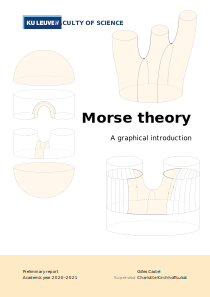
\includepdf[pages=-, fitpaper=true]{./frontmatter.pdf}
    \cleardoublepage
    \maketitle
    % \chapter*{Preface}
\label{ch:preface}
\addcontentsline{toc}{chapter}{\nameref{ch:preface}}

This thesis is on Morse theory,
the study of nice real valued functions on manifolds,
called Morse functions.
While elementary, they provide great insight in the structure of manifolds, eventually leading to some of the most important theorems in differential topology.
The goal of this thesis is to prove one of them, namely the generalized Poincaré conjecture in higher dimensions, stating that a homotopy sphere is a topological sphere.

This thesis could not have been written without the help of many people.

First and foremost, I would like to thank Dr.~Charlotte Kirchhoff-Lukat for proposing this subject and supervising me throughout my journey.
Charlotte, thank you for exposing me to the world of Morse theory and its many related topics.
Thank you for your advice, patience, and the weekly chats which kept me motivated through the year.

I would like to thank Prof.~Joeri Van der Veken and Dr.~François Thilmany for reading and evaluating this thesis.

I would like to thank my family for their support, giving me the opportunity to make this possible.

Lastly, Marie, thank you for the whiteboard in front of which we have spent many hours together.
It was essential for finishing this thesis.
Thank you for listening to my never ending rambles on Morse theory, proofreading my thesis, being the test subject for my presentations and for the much needed distraction.

\hfill \emph{Gilles, June 2021}

    \chapter*{Summary}
\label{ch:summary}
\addcontentsline{toc}{chapter}{\nameref{ch:summary}}

Morse theory is the study of smooth functions from manifolds to $\R$ that satisfy some non-degeneracy conditions. While these functions are some of the simplest things that live on manifolds, it turns out that they can provide great insight in the structure of manifolds.

In \textbf{Chapter \ref{chap:morse-theory}}, we talk about the basics of Morse theory.
We give several equivalent definitions of a Morse function and give some examples.
We also show that Morse functions give rise to so-called handle decompositions: there is a one to one correspondence between critical points of a Morse function and so-called handles, building blocks from which any manifold can be built.
We give some very concrete examples of handle decompositions in dimensions one, two and three.
We end the chapter by showing that any manifold admits (infinitely many) Morse functions.
Even more, we show that they are generic and stable, meaning that any function can be approximated by a Morse function and if we perturb a Morse function, it stays Morse.


In \textbf{Chapter \ref{chap:stable-and-unstable-manifolds}}, we introduce the concept of stable and unstable manifolds.
They form a way of understanding interaction of handles.
For example, two handles are `independent' if the intersection of their stable and unstable manifolds is empty, allowing us to reorder them, as we prove in Theorem~\label{thm:reordening}.
This idea leads to the existence of self-indexing Morse functions, asserting that we can always build a manifold by first attaching $0$-handles, then $1$-handles, $2$-handles, etcetera, in that order.
We end the chapter by proving a first cancellation theorem, stating that under certain circumstances, we can cancel pairs of critical points.

\textbf{Chapter \ref{chap:morse-homology}} concerns Morse homology.
We first define the Morse complex $C_k(f)$ and the Morse differential $\partial_X$, which is based on counting the number of trajectories along the gradient vector field $X$ between critical points of a Morse function $f$.
As an illustration, we compute some examples in two and three dimensions.
The rest of the chapter covers three important theorems in Morse theory.

First, we prove that the Morse complex is actually a complex, i.e.\ $\partial_X^2=0$.
We do this in a very detailed manner, as it is quite a subtle affair.
The geometrical idea behind this proof has inspired many other theories, for example Floer theory.

The second important result is that Morse homology is independent of the Morse function and gradient, the proof of which is arguably the most beautiful in this thesis.

Lastly, we show that Morse homology is actually isomorphic to singular homology, following the proof by Hutchings based on currents.

\textbf{Chapter~\ref{chap:app-morse-homology}} discusses some applications of Morse homology.
While we have proven that it isomorphic to singular homology, and hence it obeys all the properties singular homology enjoys, it still can be interesting to derive these facts directly from Morse homology.
For example, we can prove Poincaré duality by simply changing the Morse function $f \leadsto -f$, i.e.\ turning the manifold upside down.  This has the effect of $k$-handles becoming $n-k$-handles, flow lines reversing direction from which the desired result follows rapidly.
We also discuss the famous Morse inequalities giving a lower bound for the number of critical points of a Morse function in terms of the homology of $M$:
 \[
     \# \Crit_k f \ge \operatorname{rank} H_k(M, \Z)
.\] 
We prove some related facts including a stronger version of these inequalities.

In \textbf{Chapter~\ref{chap:h-cobord}}, we prove that under certain conditions, the Morse inequalities can be attained by some Morse function.
We prove this by considering an arbitrary Morse function,
and then cancelling pairs of critical points until the Morse inequalities have been reached.
To this purpose, this chapter mostly contains stronger cancellation results.
In Section~\ref{sec:minimality}, all these cancellation theorems come together and we prove the minimality of the Morse inequalities.
This has as an immediate corollary some of the most important theorems in differential topology: the $h$-cobordism theorem and the generalized Poincaré conjecture in dimension $n \ge 5$, stating that a homotopy sphere is a topological sphere.
Lastly, we also discuss some of the historical aspects of these theorems.

    \listofsymbols
    \tableofcontents
    \cleardoublepage
    \pagestyle{fancy}
    \renewcommand{\thepage}{\arabic{page}}
    \setcounter{page}{1}
    % \input{chaptest.tex}
    % \setcounter{chapter}{-1}
\chapter{Preliminaries}
\section*{Transversality}

\todo{Interesting source appendix of Schultens\sidecite{schultens2014introduction}}


% TODO: spell check in brackets in vim!
\begin{definition}[Transversality]
    Let $M$ be a manifold and $N_1, N_2$ be two submanifolds.
    Then $N_1$ intersects $N_2$ \emph{transversely} if and only if for all points of intersection $p \in N_1 \cap N_2$, we have
    $T_pM = T_pN_1 + T_p N_2$.
    We denote this by $ N_1 \tcap N_2$.\sidenotemark
\end{definition}
\sidenotetext{The notation is suggestive: the line $\cap$ intersects $|$ transversally: $\tcap$.}
Note in particular that this depends on the ambient manifold $M$, and that if $N_1$ and $N_2$ do not intersect, their intersection is vacuously transverse.
We give some examples below.
\begin{figure}[H]
    \centering
    \sidecaption{
        Examples and non-examples of transverse intersections.
        Multiple configurations of two circles are shown: thrice with ambient manifold $\R^2$, and once embedded in $\R^3$.
    \label{fig:transversality-examples}
    }
    \incfig{transversality-examples}
\end{figure}
A useful result is that when two manifolds intersect transversely, the codimensions of their intersection is the sum of their codimensions.
\begin{prop}
    Let $M$ be a manifold and $N_1, N_2$ be two submanifold. If $ N_1 \tcap N_2$, then 
    \[
        \codim (N_1 \tcap N_2) = \codim N_1 + \codim N_2
    ,\] 
    where the codimensions relative to $M$.
    \label{prop:transverse-codimensions-add}
\end{prop}
\begin{proof}
    As this is a local statement, we prove it for $M = \R^{m}$.
    We may assume that $N_1 = f_1^{-1}(0)$ and $ N_2 = f_2^{-1}(0)$ where $f_i$ are submersions from $\R^{m}$ to $\R^{n_i}$, where $n_i$ is the codimension of $N_i$.
    % i.e. $(f_i)_*$ has full rank everywhere.
    \begin{marginfigure}
        \centering
        \incfig{codimensions-transverse}
        \caption{When $N_1 \tcap N_2$, the codimension of the intersection is the sum of their codimensions. By using the implicit function theorem, we straighten the situation.}
        \label{fig:codimensions-transverse}
    \end{marginfigure}
    Then we can also consider $F= (f_1, f_2): \R^{m} \to  \R^{n_1} \times \R^{n_2}$.
    Notice that $ N_1 \cap N_2 = F^{-1}(0)$.
    Then
    \begin{align*}
        \dim N_1 \cap  N_2 &= \dim \Ker d_0F\\
                           &= \dim(\Ker d_0 f_1 \cap \Ker d_0 f_2)\\
                           &= \dim \Ker d_0 f_1 + \dim \Ker d_0 f_2 - \dim (\Ker d_0 f_1 + \Ker d_0 f_2)\\
                           &= (m - n_1) + (m - n_2) - m\\
                           &= m - (n_1 + n_2)
    .\end{align*} 
    This completes the proof.
\end{proof}
Note that this proof also shows that $T_p(N_1 \tcap N_2) = T_pN_1 \tcap T_pN_2$ and that $ N_1 \tcap N_2$ is a manifold, which is not always the case when the intersection is not transverse.

\begin{marginfigure}
    \centering
    \incfig{intersection-of-manifolds-is-not-always-a-manifold}
    \caption{Let $M = \R^2$ and let $N_1$ and $N_2$ be submanifolds as in the figure. Then $N_1$ and $N_2$ do not intersect transversely and their intersection is not a manifold: it is the union of a point and a closed interval.}
    \label{fig:intersection-of-manifolds-is-not-always-a-manifold}
\end{marginfigure}

\begin{theorem}[Sard's theorem]
    Let $f: M \to  N$ be a $\Cinfty$ map. Then the set of critical values of  $f$ has measure zero in $N$.
\end{theorem}
\begin{proof}
    Omitted.
\end{proof}



\begin{definition}[Isotopy\sidenotemark]
    Two embeddings $f_0, f_1: M \to  N$ are \emph{isotopic} if there is a continuous map $H: M \times  [0, 1] \to  N$ such that $H(x, 0) = f_0$ and $H(x, 1) = f_1(x)$ for all $x \in M$ and such that for all $t \in [0, 1]$, the map $f_t$ defined by $H(\cdot , t)$ is an embedding. The map $H$ is called an \emph{isotopy between} $f_0$ and $f_1$.

    Two submanifolds $S_0, S_1$ of $M$ are \emph{isotopic} if their inclusion maps are isotopic.
\end{definition}
\sidenotetext{\fullcite[23]{schultens2014introduction}}

    % \chapter{Morse theory}

When studying manifolds is often proves useful to study simple structures that live on them. For example, studying differential forms gives rise to the de Rham cohomology, which tells us something about the global structure of the manifold. In this thesis, we study some of the most simple maps: maps from the manifold $M$ to $\R$. A prototypical example of such a map is a projection.
While these projections seem to lose much information, we will see that they actually can provide great insight in the structure of the manifold itself.

\section{Definition of a Morse function}

We will not consider arbitrary maps $M \to \R$, but rather maps that have nice behaviour at their critical points. Let us first recall what a critical point is.

\begin{definition}[Critical point]
    Let $M$ and $N$ be a manifolds and  $f$ a map from $M$ to $N$.
    The critical points of $f$ is the set given by
    \[
    \Crit f = \{p \in M  \mid \text{$df_p$ is not surjective}\} 
    .\] 
    In particular, if $N = \R$ we have that
    \[
    \Crit f = \{ p \in M  \mid  df_p = 0\} 
    .\] 
\end{definition}
The maps we will be considering are then characterised as follows:
\begin{definition}[Morse function]
    Let $M$ be a manifold. A function $f: M \to  \R$ a \emph{Morse function} if for all critical points $p$, there exists a chart centred around $p$ such that $f$ is locally given by
    \[
        f(x) = f(p) -x_1^2 - \cdots - x_k^2 + x_{k+1}^2 + \cdots + x_n^2
    .\] 
    We call such a chart a \emph{Morse chart} and we call $k$ the index of $p$, which we also denote with $\Ind p$.
    
\end{definition}
Intuitively, the index of a critical point $p$ is ``the number of downward directions''.
Let us first give some examples.
\begin{marginfigure}
    \centering
    \incfig{examples-of-morse-functions}
    \caption{Example of a Morse function on the torus. At each critical point, the index $k$, the number of downward directions is indicated. }
    \label{fig:examples-of-morse-functions}
\end{marginfigure}
\begin{eg}
    Let $M$ be the torus  $T^2$ embedded in $\R^3$ as illustrated in Figure~\ref{fig:examples-of-morse-functions}.
    Then the height function $h: T^2 \to  \R$ which is the projection on the $z$-axis is a Morse function with four critical points:
    \begin{itemize}
        \item A minimum $p$, where $h(x) = h(p) + x_1^2 + x_2^2$.
        \item Two saddle points $s_1, s_2$ where $h(x) = h(s_i) + x_1^2 - x_2^2$.
        \item A maximum $q$ where $h(x) = h(q) - x_1^2 - x_2^2$.
    \end{itemize}
\end{eg}

\begin{noneg}
    Let $M = \R^2$ and $f: \R^2 \to  \R: (x, y) \mapsto  x^2$.
    Then all points $(0, y)$ for  $y \in \R$ are critical points of this function.
    In particular, $(0, 0)$ is a critical point. Locally, we cannot write $f$ as  $ \pm x_1^2 \pm x_2^2$ for some coordinates $(x_1, x_2)$, so $f$ is not Morse.
\end{noneg}
\begin{marginfigure}
    \centering
    \incfig{non-example-of-morse-function}
    \caption{}
    \label{fig:non-example-of-morse-function}
\end{marginfigure}
\begin{marginfigure}
    \centering
    \incfig{non-examples-of-morse-functions}
    \caption{An example of a function that is not Morse: $f: \R \to  \R: x \mapsto  x^3$.
        Small perturbations of $f$ are Morse.
    }
    \label{fig:non-examples-of-morse-functions}
\end{marginfigure}
\begin{noneg}
    Let $M = \R$ and $f : \R \to  \R: x \mapsto x^3$.
    Then $x = 0$ is a critical point, but $f$ is not Morse.
    Note however that if we add a small perturbation to $f$, say $g_t: x\mapsto x^3+ tx$, then for small non-zero $t$, $g$ is Morse. For $t < 0$, $g_t$  has two critical points: one of index $1$ and one of index $0$.
    If $t > 0$,  $g_t$ has no critical points.
\end{noneg}

Note that this last case where $f$ has no critical points cannot happen if $M$ is compact.
Indeed, any function attains it maximum and minimum on a compact manifold, so we have at least two critical points.
On the other hand, the number of critical points is at most finite.
This is because of the definition of a Morse function: it implies that critical points are isolated, which on a compact manifold implies that their number is finite.
This also immediately rules out the situation we had in the other example, where the set of critical points was a straight line.

\section{Coordinate-free definition of a Morse function}

The attentive reader will have noticed that the definition of the index of a critical point could possibly not be well defined.
To show that it is and that $\Ind p$ does not depend on the choice of coordinates, we will will give a coordinate-free definition. For this, we first need to define the Hessian at a critical point.

\begin{definition}
    Let $M$ be a manifold and $f: M \to  \R$ a function.
    Let $p$ be a critical point of $f$.
    Then we define the Hessian $H_p$ to be the bilinear form
    \begin{align*}
        H_p: T_pM \times T_pM &\longrightarrow  \R\\
        (X, Y) &\longmapsto X (\tilde{Y} f)|_p
    ,\end{align*} 
    where $\tilde{Y}$ is a local extension of $Y$ around $p$.
\end{definition}
This is a well defined symmetric bilinear form.\sidenote{The difference between $H_p(X, Y)$ and  $H_p(Y, X)$ is given by
\begin{align*}
    H_p(X, Y) - H_p(Y, X) &= X(\tilde{Y} f)|_p - Y (\tilde{X} f)|_p\\
                          &= [\tilde{X}, \tilde{Y}] f |_p\\
                          &= df_p [\tilde{X}, \tilde{Y}]|_p = 0
.\end{align*}
The value of $H_p$ also does not depend on the extension of the vector field.
Indeed, suppose $\tilde{Y}$ and $\overline{Y}$ are two different extensions of $Y$. Then by symmetry of $H_p$, we have
\[
    X(\tilde{Y} f)|_p = Y(\tilde{X} f)|_p = X(\overline{Y}f )|_p
.\] 
This also shows linearly of the second component.
}
In case of a Morse function given locally by $f(x) = f(p) - x_1^2 - \cdots - x_k^2 + x_{k+1}^2 + \cdots + x_n^2$, the Hessian at $p$ is 
\[
    H_p = 2(- dx_1^2 - \cdots - dx_k^2 + dx_{k+1}^2  + \cdots + dx_n^2)
,\] 
where $dx_i^2 = dx_i \otimes dx_i$.
Note in particular that $H_p$ is non-degenerate and its signature is $(i_-, i_{+}) = (k, n-k)$, as we have $k$ negative eigenvalues, $n-k$ positive eigenvalues.
As the signature of a symmetric bilinear form is coordinate independent, this shows that the index of a critical point is as well.


Interestingly, the reverse is also true: if $H_p$ is non-degenerate for all critical points  $p$ of $f$, then  $f$ is a Morse function.
Many authors take this to be the definition of a Morse function.

\begin{lemma}[Morse Lemma]
    Let $M$ be a manifold and $f: M \to  \R$ a smooth map.
    If for all $p \in \Crit f$, the Hessian $H_p$ is non-degenerate, then $f$ is Morse.
\end{lemma}
\begin{proof}
    We follow the proof of Milnor\sidecite[6]{milnor}.
    We may assume that $M = \R^{n}$, $p$ is the origin and $f(p) = 0$.
    Then by a version of Taylor's theorem, we can write
    \begin{align*}
        f(x)  &= f(p) + \sum_{i=1}^{n} (x_i - p_i) g_i (x)\\
              &= \sum_{i=1}^{n} x_i g_i(x)
    ,\end{align*} 
    where $g_i$ are smooth functions. 
    Now, as $g_i(0) = \partial_i f (0) = 0$, we can repeat this for each  $g_i$, giving us the following:
    \[
        f(x) = \sum_{i, j= 1}^{n} x_i x_j h_{ij}(x)
    .\] 
    Because this sum is symmetric in $i$ and  $j$, we may assume that  $h_{ij}$ is symmetric as well.\sidenote{If $h_{ij}$ is not symmetric, we can replace it by $h_{(ij)} = \frac{1}{2}(h_{ij} + h_{ji})$. Then $h_{(ij)}$ is symmetric and we still have $\sum x_{i}x_{j}h_{ij} = \sum x_{i}x_{j}h_{(ij)}$.}
    Note that
    \[
        h_{ij}(0) = \frac{1}{2} \partial_{ij} f(0)
    ,\]
    which is non-degenerate by assumption.

    Now we imitate the proof of diagonalization of a non-degenerate quadratic form.
    We do this by induction.
    Suppose we have coordinates $u_1, \cdots, u_n$ in a neighbourhood of $0$ such that
    \[
        f = \pm u_1^2 \pm \cdots \pm u_{r-1}^2 + \sum_{i,j\ge r} u_i u_j H_{ij}(u)
    ,\] 
    where $H_{ij}$ is a symmetric matrix.
    After a linear change, we may assume by non-degeneracy that $H_{rr} \neq 0$.
    Then define new coordinates $ v_1, \ldots, v_r$ as follows:
    \[
        v_i = \begin{cases}
            u_i & \text{if $i \neq r$}\\
            \sqrt{|H_{rr}|} (u_r + \sum_{i > r} u_i H_{ir} / H_{rr}) & \text{if $i = r$.}
        \end{cases}
    \] 
    Note that we may need to restrict the neighbourhood such that $\sqrt{H_{rr}} \neq 0$.
    Then we have that
    \[
        f = \sum_{i\le r} \pm v_i^2 + \sum_{i,j > r} v_i v_j H_{ij}'(v)
    .\] 
    for some symmetric matrix $H_{ij}'$.
    \todo{Explain better}
    % Indeed,
    % \begin{align*}
    %     v_r^2 &= |H_{rr}| \left(u_r^2 + \sum_{i>r} 2 u_r u_i H_{ir} / H_{rr} + \left(\sum_{i>r} u_i H_{ir} / H_{rr}\right)^2\right)\\
    %           &= TODO
    % .\end{align*} 

\end{proof}

\section{Handle decompositions}
\todo{Introduction}

\todo{Check definition Milnor $h$-cobordism and fix definition Morse function}
\begin{definition}
A cobordism between two compact manifolds $M_1$ and $M_2$ is a compact manifold $M$  with boundary $\partial M = M_1 \sqcup M_2$.
\end{definition}


The term `cobordism' comes from the fact that $M_1 \sqcup M_2$ are the boundary of $M$, so we can think of $M$ as the `co-boundary' of $M_1$ and $M_2$.
Cobordisms are an interesting topic in their own right.
For example, they define an equivalence relation on all compact manifolds of same dimension. Two manifolds $ M_1$ and $M_2$ are then said to be equivalent (cobordant) if there exists a cobordism $M$ connecting the two.
This equivalence relation is coarser than diffeomorphism and is generally easier to study.
Cobordisms also form a category where the objects are manifolds and the arrows are cobordisms.

We have illustrated some examples below.
Note that we may also take $M_1$ or $M_2 = \O$.
In particular, any closed manifold is a cobordism from $\O$ to $\O$.
\begin{figure}[H]
    \centering
    \sidecaption{Some examples of cobordisms. 
        When the height function has a critical point, the topology changes from top to bottom.
    \label{fig:examples-of-cobordisms} }
    \incfig{examples-of-cobordisms}
\end{figure}

When we consider the height function $f: M \to  [0, 1]$ on these examples,
we observe that the topology of the bottom is different than that of the top if the height function has critical points.
This is indeed in general true.
If $f$ is a Morse function (as is the case in our examples), it will turn out we can very concretely describe \emph{how} this topology changes.
This will give rise to the concept of handle decompositions.

\newthought{Let us first consider} the case where $f: M \to [0, 1]$ has no critical points. 
For simplicity, we introduce the following refined definition of a Morse function on a cobordism:
\begin{definition}[Morse function on a cobordism\sidenotemark]
    Let $M$ be a cobordism from $M_0$ to $M_1$.
    A function $f: M \to  [a, b]$ is said to be \emph{Morse} if 
    \begin{itemize}
        \item $M_0 = f^{-1}(a)$, $M_1 = f^{-1}(b)$
        \item All critical points lie interior in $M$ and are non-degenerate.
    \end{itemize}
\end{definition}
\sidenotetext{\fullcite[8]{hcobord}}

\begin{prop}
    Suppose $f: M \to  [a, b]$ is a Morse function on a cobordism $M$ from  $ M_0$ to $ M_1$.
    If $f$ has no critical points, then $M$ is diffeomorphic to $[a, b] \times  M_0$.
\end{prop}
\begin{proof}
    \todo{Check proof $h$-cobordism milnor}
    \begin{marginfigure}
        \centering
        \incfig{proof-of-cobordism-without-critical-points}
        \caption{
            When a cobordism has no critical points, it is diffeomorphic to a product manifold. }
        \label{fig:proof-of-cobordism-without-critical-points}
    \end{marginfigure}
    Consider a Riemannian metric $\left<\cdot ,\cdot  \right>$ on $M$.
    Because  $f$ has no critical points, the vector field $W = (df)^{\sharp}$ never vanishes.\sidenote{Here and hereafter, we use $\sharp$ and $\flat$ for the `musical isomorphisms' induced by metric $\left< \cdot, \cdot \right>$, given by
        \begin{align*}
            \flat: TM \longrightarrow T^*M: &\:X \longmapsto X^{\flat} = \left<X, - \right>\\
            \sharp: T^*M \longrightarrow TM :&\:\alpha \longmapsto \alpha^{\sharp}
        ,\end{align*}
        where $\alpha^\sharp$ is uniquely defined by $\langle\alpha^\sharp, X\rangle = \alpha(X)$.
    }
    Consider the normalized vector field
    \[
    V = \frac{1}{\left<W, W \right>} W
    .\] 
    Then $df(V) = \frac{1}{\left<W, W \right>} df(W) = 1$.
    Consider
    \begin{align*}
        \phi: [0, 1] \times M_0&\longrightarrow M \\
        (t, p) &\longmapsto \theta_V^{t}(p)
    ,\end{align*}
    where $\theta_V^{t}$ is the flow along $V$.
    Then $f(\phi(t, p)) = t$ for all $p \in M_0$, as $df(V) = 1$.
    The map $\phi$ is injective because of the uniqueness of flows, and surjective because given a point $p$ in $M$, we can always flow back along $V$ for a time $t$ to find a $p_0 \in M_0$ which then satisfies $\phi(t, p_0) = p$. 
    This also proves that $\phi$ is a diffeomorphism.
\end{proof}
This result is very useful and is sometimes used to prove that two manifolds $M_0$ $M_1$ are diffeomorphic: if we can construct a cobordism from $M_0$ to $M_1$ and we can prove the existence of a Morse function without critical points, then $M_0 \cong M_1$.


\todo{Corollary: collar and bicollar theorem. Milnor $h$-coboridsm.}
\todo{Corollary: we can glue two cobordisms together and get a manifold un a unique way. Milnor $h$-coboridsm.}

In the case in which $f$ does have a critical point $p$, the previous proof fails because $d_pf = 0$, so $\grad f = (df)^{\sharp}$ vanishes at some point.


\newthought{Let us now investigate} the situation when a Morse function $f$ does have a single critical point, say $p$ and assume $f(p) = 0$.
Then we know $f$ is locally of the following form:
\[
    f(x_1, \ldots, x_n) = - x_1^2 - \cdots - x_k^2 + x_{k+1}^2 + \cdots + x_n^2
.\] 
In Figure~\ref{fig:morse-chart}, we have plotted the first $k$ variables (the `downward directions') on the horizontal axis, and the last $n-k$ variables on the vertical axis.
Then the level set $f^{-1}(0)$ is given by
\[
x_1^2 + \cdots + x_k^2 = x_{k+1} ^2 + \cdots + x_n^2
,\] 
which consists of the two crossing lines in the figure, corresponding to the crossing part of the figure-eight on the right.
Level sets of values slightly above an below $0$ look locally like hyperbolas on our figure, but remembering that that the axes consist of multiple dimensions, it would be more precise to call them hyperboloids.

\todo{Add figure movie: two hyperbolas switching, hyperboloids, one handle in three dimensions that joins, \ldots}
\begin{figure}[H]
    \centering
    \sidecaption{Around a critical point of a Morse function, we can find a chart as on the left. The dark region corresponds to $f(x) < 0$, the light region to $f(x) >0$. The level set $f^{-1}(0)$ is not a manifold.
    \label{fig:morse-chart}}
\incfig{morse-chart}
\end{figure}

To contain the behaviour of the critical point, it is useful to cut out the area bounded by the level sets $f = \pm \epsilon$ in order to make it compact.\todo{wording}.
A natural way to do this, is to cut along gradient flow lines of $f$ (Figure~\ref{fig:morse-chart-flow-lines} and \ref{fig:morse-chart-zoomed-in}).
Of course, a gradient is only defined when we have a metric, and here we choose to use the standard metric on $\R^{n}$.\sidenote{More explicitly, if $f$ is Morse, we know that locally around a critical point $p$, $f$ is given by
    \begin{align*}
        f(x_1, \ldots, x_n) &= f(p) - x_1^2 - \cdots - x_k^2\\
                            & \qquad + x_{k+1}^2 + \cdots + x_n^2
    .\end{align*} 
    Then the negative gradient of $f$ w.r.t.\ the standard metric on $\R^n$ is
    \begin{align*}
        - \grad f &= 2 x_1 \partial_{1} + \cdots + 2 x_k \partial_{k}\\
                & \qquad - 2 x_{k-1} \partial_{k-1} - \cdots - 2 x_n \partial_{n},
    \end{align*}
    where $\partial_i = \partial_{x_i}$.
} In Morse theory it is also customary to consider the negative gradient instead of the standard one.
\begin{marginfigure}
    \centering
    \incfig{morse-chart-flow-lines}
    \caption{A Morse chart with negative gradient flow lines added.
    The coloured area represents a handle. Its boundary consists of parts of level sets of $f$ and flow lines of $\grad f$.}
    \label{fig:morse-chart-flow-lines}
\end{marginfigure}
In Figure~\ref{fig:morse-chart-zoomed-in}, the cut out area is coloured in yellow.
The advantage of cutting along gradient flow lines, is that we have split up the cobordism in three parts which we understand well:
\begin{marginfigure}
    \centering
    \incfig{morse-chart-zoomed-in}
    \caption{A cobordism with one critical point splits up in product structures and a handle.}
    \label{fig:morse-chart-zoomed-in}
\end{marginfigure}
\begin{itemize}
    \item[\circled{A}] The part below $-\epsilon$ and the part above $\epsilon$ have a product structure, because we assumed the only critical value was $0$.
        We can simply repeat the proof above.
    \item[\circled{B}] The part of $M$ that lies between $-\epsilon$  and $\epsilon$ without $\circled{H}$ also has a product structure.
        To see this, extend the metric on $\circled{H}$ to the whole manifold. Then, because $f$ has no critical values outside $\circled{H}$, we can flow along gradient lines giving us a product structure.
        This is why we cut in this way: we want the boundary of this region to consist of gradient lines, or the proof would fail.

        Riemannian metrics are an extension of standard metrics around critical points are called adapted Riemannian metrics.
        Using a partition of unity argument, one can show any manifold admits such metrics.
        \begin{definition}[Adapted Riemannian metric]
            A Riemannian  metric is called \emph{adapted} to a Morse function $f$ if near all its critical points $p \in \Crit f$, the metric is locally, in each Morse chart given by
            \[
            \left<
            (x_1, \ldots, x_n), 
            (y_1, \ldots, y_n)
            \right> = \sum x_i y_i
            .\] 
        \end{definition}
        In most cases, we often forget about the metric itself and simply consider vector fields which are gradient-like.

        \begin{definition}[Pseudo-gradient]
            Let $f: M \to  \R$ be a Morse function on a manifold $M$. A pseudo-gradient is a vector field $X$ such that
            \begin{itemize}
                \item $df(X) \le 0$ and $df(X) = 0$ only at critical points
                \item $X$ coincides in Morse charts with the usual negative gradient for the standard metric on $\R^{n}$.
            \end{itemize}
        \end{definition}




    \item[\circled{H}]  The yellow part is what we call a \emph{handle of index $k$}, and is homeomorphic to $\disk{k} \times \disk{n-k}$.
        This is the only non-trivial part of our cobordism.
        We call the bottom part of the border the \emph{attachment region}, which is homeomorphic to $S^{k-1} \times \disk{n-k}$.
\end{itemize}






\newthought{If a Morse function} on a cobordism has multiple critical points, then we can always assume that the critical values are distinct and isolated.
We can do this by adding a small perturbation to $f$.\todo{prove this}.
Then we can split up the cobordism in parts having only one or zero critical points, and decompose each part in products and handles like before.

As any closed manifold can be viewed as a cobordism from $\O$ to $\O$, we have proved the following:

\begin{theorem}
    Any closed manifold has a handle decomposition.
\end{theorem}

Before discussing some examples, let us first discus some of the different ways to look at handles.
\todo{Add subtleties about corners, \ldots
Thickened up intervals.
Instead of having morse function and decomposing, you can also ask question how you can build a manifold?

Embed attachment region in the manifold you already have.}


\subsection*{Handles in low dimensions}

In this section, we will consider some examples of handle decompositions in dimension one, two and three.

\newthought{Handles in dimension one} are the most simple ones. We only have two types:

\begin{description}
    \item[0-handle] $\disk0 \times \disk{1} = [-1, 1]$, with attachment region $\O$. \hfill \minifig{1cm}{handle-1-0} 
        
    \item[1-handle]   $\disk{1} \times  \disk{0} = [-1, 1]$ with attachment region $S^{0} = \{-1, 1\}$.  \hfill \minifig{1cm}{handle-1-1}
\end{description}

\begin{eg}
    In Figure~\ref{fig:one-dimensional-handle-decomposition-examples}, two handle decompositions of $S^{1}$ are illustrated.
    The first one is based on the height function $f$ when embedding $S^{1}$ in $\R^2$.
    For the second decomposition, $g$ is again defined as a height function, but this time we embedded $S^{1}$ in $ \R^2$ in a non-standard way.
    This way, we get two different handle decompositions of the same manifold.
\end{eg}
\begin{figure}[H]
    \centering
    \sidecaption{Two handle decompositions of $S^{1}$.
    \label{fig:one-dimensional-handle-decomposition-examples}}
    \incfig{one-dimensional-handle-decomposition-examples}
\end{figure}
This example illustrates that handle decompositions are not unique.
However, we can construct an isotopy from the second to the first embedding that cancels the two critical points.
Interestingly, the height function is Morse for all $t$, except at the exact moment when the cancellation happens.
A local model for this is $t\mapsto x^3 + tx$ as in Figure~\ref{fig:non-examples-of-morse-functions}.
\begin{figure}[H]
    \centering
    \sidecaption{There exists an isotopy between the two handle decompositions described above.
    \label{fig:isotopy-between-circle-and-other-circle}}
    \incfig{isotopy-between-circle-and-other-circle}
\end{figure}


\paragraph{Handles in dimension two}
In dimension two, things get more interesting.
We have three types of handles:
\todo{Mention somewhere homology group changes when adding handles. But handle decomposition is not unique, if we could mod out these critical points which can cancel, then it is unique? Giving rise to Morse complex.}

\begin{description}
    \item[0-handle] $\disk{0} \times \disk{2}$ with attachment region $\O$. \hfill \minifig{1cm}{handle-2-0}
    \item[1-handle] $\disk{1} \times \disk{1}$ with attachment region $\disk1 \times S^{0}$. \hfill\minifig{1cm}{handle-2-1}
    \item[2-handle] $\disk{2} \times \disk{0}$ with attachment region $\disk{0} \times S^1$. \hfill\minifig{1cm}{handle-2-2}
\end{description}

\begin{eg}[Handle decomposition of the torus]
    Consider the height function on the torus embedded in $\R^3$. This Morse function gives rise to the handle decomposition in Figure~\ref{fig:handles-in-dimension-two-torus-decomposition}: a $0$-handle, two $1$-handles and one $2$-handle.
\end{eg}

\begin{marginfigure}
    \centering
    \incfig{handles-in-dimension-two-torus-decomposition}
    \caption{The standard embedding of the torus in $\R^3$ gives rise to a handle decomposition consisting of one  0-handle, two 1-handles and three 2-handles.}
    \label{fig:handles-in-dimension-two-torus-decomposition}
\end{marginfigure}

\begin{eg}[The `other sphere']
    In Figure~\ref{fig:handles-in-dimension-two-other-sphere}, an embedding of $S^2$ in $\R^3$ is given, and we again consider the height function.
    This function is Morse, and gives rise to a handle decomposition with a $0$-handle, a $1$-handle and two $2$-handles.
\end{eg}
\begin{marginfigure}
    \centering
    \incfig{handles-in-dimension-two-other-sphere}
    \caption{Embedding $S^2$ in $ \R^3$ in an unusual way gives rise to a handle decomposition with one 0-handle, one 1-handle and two 2-handles. }
    \label{fig:handles-in-dimension-two-other-sphere}
\end{marginfigure}



\paragraph{Handles in dimension three}

\todo{Mention that sometimes you cannot attach handle before other one. When \emph{is} it possible? Hint to descending manifold, \ldots}

\begin{description}
    \item[0-handle] $ \disk0 \times \disk{3}$ with attachment region $\O$ 
        \hfill\minifig{1cm}{handle-3-0}
    \item[1-handle] $ \disk1 \times \disk{2}$ with attachment region $ \disk2 \times S^{0}$
        \hfill\minifig{1cm}{handle-3-1}
    \item[2-handle] $ \disk2 \times \disk{1}$ with attachment region $ \disk1 \times S^1$
        \hfill\minifig{1cm}{handle-3-2}
    \item[3-handle] $ \disk3 \times \disk{0}$ with attachment region $S^{2}$
        \hfill\minifig{1cm}{handle-3-3}
\end{description}

Drawing three-dimensional handle decompositions is a bit harder. Most of the times we suppress the $0$-handle, and also the $3$-handle is not drawn. If a $3$-handle is to be attached, we usually write ``$\cup $ $3$-handle''

\begin{eg}[Handle decomposition of $S^{3}$]
    Consider $S^{3} \subset \R^{4}$ and the height function $f$, the projection on the last coordinate.
    Then $f$ has two critical points: $(0, 0, 0, \pm 1)$ of index $0$ and $3$.
    Then handle decomposition is then a $0$-handle ($\disk{3}$) glued to a $3$-handle (which is also diffeomorphic to $\disk{3}$).
\end{eg}

\begin{eg}[Handle decomposition of $ S^1\times S^{2}$]
    An example of a handle decomposition of $S^{1} \times S^{2}$ is illustrated in Figure~\ref{fig:handles-in-dimension-three-s1-x-s2}.
    The construction starts with a $0$-handle, which is just a three dimensional ball.
    Then we glue on a $2$-handle.
    The resulting manifold is then a thickened-up \todo{spelling}  two sphere, $I \times S^{2}$.
    Then we add a $1$-handle connecting the inside to the outside and we cap of with a $3$-handle, which has the effect of identifying the end points of $I$, i.e. this transforms  $I \times S^{2}$ into $ S^1 \times S^{2}$.
\end{eg}
\begin{marginfigure}
    \centering
    \incfig{handles-in-dimension-three-s1-x-s2}
    \caption{Top: $ S^1 \times S^{2}$ can be decomposed using a 0-handle, 1-handle, 2-handle and 3-handle.
        Bottom: same handle decomposition, but drawn differently to show that  a 0-handle and a 1-handle are diffeomorphic to $S^{2} \times [0,1]$.
}
    \label{fig:handles-in-dimension-three-s1-x-s2}
\end{marginfigure}

\begin{eg}
    \todo{Example of a $1$ and $2$-handle that collapse. }
\end{eg}
\begin{eg}[$T^{3} = S^{1} \times S^{1} \times S^{2}$]
    \label{eg:handle-decomposition-three-torus}
    To find a handle decomposition of $T^3$, we identify $T^{3}$ with $\R^3 / \Z^{3}$ and consider the following map
    \begin{align*}
        f: T^{3} &\longrightarrow \R \\
        (x, y, z) &\longmapsto 2\cos (2 \pi x) + 3\cos ( 2 \pi y) + 4 \cos(2 \pi z)
    .\end{align*}
    Then we have
    \[
        df =
        -4\pi \sin (2 \pi x) dx
        -6 \pi \sin ( 2 \pi y) dy
        - 8 \pi \sin(2 \pi z) dz
    ,\] 
    so critical points are all $(x, y, z) \in \R^3 / \Z^3$ for which  $x, y, z \in \left\{\Z, \frac{1}{2} + \Z\right\}$.
    In total we have $8$ distinct critical points, and they all are non-degenerate, because the Hessian of $f$, given by
    \[
        H_{(x, y, z)} f =
        - 8 \pi^2  \cos (2 \pi x) dx^2
        -12\pi^2 \cos ( 2 \pi y) dy^2
        -16 \pi^2 \cos(2 \pi z) dz^2
    \] 
    is non-degenerate at each of the critical points.
    To find the handle decomposition induced by $f$, we have to determine the index of the critical points.
    As discussed earlier, the index is the number of downward directions, which is also equivalent to the number of negative eigenvalues of $H_{(x, y, z)}f$.
    As $\cos(2 \pi \frac{1}{2}) < 0$ and $\cos(2 \pi 0) > 1$, we find that the index of a critical point $(x, y, z)$ is the number of zeros occurring in the triplet $(x, y, z)$. Hence, we get the following table:
    \[\begin{array}{cccccc}
  & x & y  & z & f(x, y, z) & \text{Index}\\ \hline
  & 0 & 0 & 0 & 9 & 3 \\
& \frac{1}{2} & 0 & 0 & 5 & 2 \\
& 0 & \frac{1}{2} & 0 & 3 & 2 \\
& 0 & 0 & \frac{1}{2} & 1 & 2 \\
& \frac{1}{2} & \frac{1}{2} & 0 & -1 & 1 \\
& \frac{1}{2} & 0 & \frac{1}{2} & -3 & 1 \\
& 0 & \frac{1}{2} & \frac{1}{2} & -5 & 1 \\
& \frac{1}{2} & \frac{1}{2} & \frac{1}{2} & -9 & 0 \\
    \end{array}\]
    We conclude that we can decompose $T^3$ in one $0$-handle, three $1$-handles, three $2$-handles and one $3$-handle.

    A natural question that arises is: `Can we build $T^{3}$ using less handles'?
    \todo{Mention that values of critical points are not distinct}


    \todo{Explain and make full page width}
    \begin{figure}[H]
    \centering
    \incfig{three-torus-handle-decomposition}
    \caption{
        Step by step construction of $T^{3}$ adding one handle at the time.
        Here, $T^{3} = \R^3/ \Z^3$, and $\left[-\frac{1}{2}, \frac{1}{2}\right]^3$ is drawn.
        The construction starts with a $0$-handle.
        In the first three steps, a $1$-handle is added.
        In the consequent steps,
        three holes are filled with $2$-handles,
        leaving us with a single void we fill up with a $3$-handle.
    }
    \label{fig:three-torus-handle-decomposition}
\end{figure}
\end{eg}




\section{Existence and abundance of Morse functions}
One might think that Morse functions are very specific functions and hence they form a small subset of all smooth maps $M \to  \R$.
In this section we show that this is not the case. We will show that any manifold admits uncountably many Morse functions and that the set of Morse function form a dense subset of all smooth maps $M \to  \R$.

Let us first recall the following result, due to Withney\sidecite{todo}.
\begin{theorem}[Withney Embedding Theorem]
    Any smooth manifold $M$ of dimension $m$ can be embedded into  $\R^{2m+1}$
\end{theorem}
This allows us to assume that $M$ is diffeomorphic to a submanifold $V$ of $\R^{n}$, making the constructions  more straightforward.
The following theorem says that there is an abundance of Morse functions on any manifold.
\begin{marginfigure}
    \centering
    \incfig{level-sets-of-distance-function-torus}
    \caption{An embedding of the torus $T^2$ in $\R^3$. The level sets of $f_p$ are spheres. We see that $f_p$ has four critical points: a maximum, a minimum and two saddle points.}
    \label{fig:level-sets-of-distance-function-torus}
\end{marginfigure}
\begin{prop}
    Let $V \subset \R^{n}$ be a submanifold.
    Then for almost every point $p \in \R^{n}$, we have that
    \[
    f_p : V \to \R: x \mapsto  \|x - p\|^2
    \] 
    is a Morse function.
\end{prop}


First, let us give an example of when $f_p$ is \emph{not} a Morse function.

\begin{marginfigure}
    \centering
    \incfig{example-when-fp-is-not-a-morse-function}
    \caption{When $p$ is the center of a circle, $f_p$ is not a Morse function}
    \label{fig:example-when-fp-is-not-a-morse-function}
\end{marginfigure}
\begin{eg}
    Let $V = S^1 = \{\|x\|^2 = 1  \mid  x \in \R^2\} $.
    Then $f_{(0, 0)}$ is not a Morse function.
    Indeed, $f_{(0, 0)} \equiv 1$, so in particular the second derivative is non-degenerate (it vanishes everywhere).
\end{eg}


More generally, $f_p$ is not a Morse function when infinitesimally close normals intersect in $p$, because then $f_p$ is constant up to second order (\todo{in a certain direction \ldots }).
To make this exact, we will show that $H_p$ is non-degenerate if $p$ is a critical value of the map
\[
    E: NV \to  \R^{n}: (x, v) \mapsto x + v
,\]
where $N$ is the normal bundle of $V$.
Then Sard's theorem\sidecite{todo} will immediately imply that $f_p$ is Morse for almost all $p$.

\begin{figure}[H]
    \centering
    \sidecaption{
        Visualization of the normal bundle of $V$, a submanifold of $\R^n$, and the map $E$ used in the proof.
    }
    \incfig{existence-of-morse-functions-normal-bundle-map}
    \label{fig:existence-of-morse-functions-normal-bundle-map}
\end{figure}

\begin{proof}
    Given this insight, the proof now reduces to a straightforward calculation.
    First note that $x$ is a critical point of $f_p$ only if $x-p \perp T_x V$.
    Indeed:
    \[
        d f_p = \sum d(x_i - p_i)^2 = 2 \sum (x_i-p_i) dx_i = 0 \qquad \text{if $x-p \perp T_x V$}
    .\] 
    Let $d = \dim V$ and $(u_1, \ldots, u_d) \mapsto x(u_1, \ldots, u_d)$ be a local parametrization of $V$.
    Then we have
    \[
        \partial_i f_p = 2(x-p) \cdot  \partial_i  x
    \] 
    and for the hessian we have
    \[
    H_p = \partial_{ij} f_p = 2 \left(\partial_j x \cdot \partial_i x  + (x-p) \partial_{ij} x \right)
    ,\] 
    where we denoted $\partial_i = \frac{\partial }{\partial u_i}$.
    We will show that $H_p$ is not of full rank if and only if $p$ is a critical value of  
    \[
        E: NV \to  \R^n: (x, v) \mapsto x + v
    ,\] 
    where $NV$ is the normal bundle to $V$ w.r.t.\ the Euclidean metric on $\R^n$.

    First we define a local parametrization of $NV$:
    \[
        (u_1, \ldots, u_d, t_1, \ldots, t_{n-d}) \mapsto \Big(x(u_1, \ldots, u_d), \sum_{i=1}^{n-d} t_i v_i(u_1, \ldots, u_{d})\Big)
    ,\] 
    where the $v_i$ form a local orthonormal basis at each point, normal to $TV$.
\begin{marginfigure}
    \centering
    \incfig{abundance-of-morse-functions-parametrization-of-the-normal-bundle}
    \caption{Parametrization of the normal bundle of $V$.}
    \label{fig:abundance-of-morse-functions-parametrization-of-the-normal-bundle}
\end{marginfigure}
    Then in these coordinates,
    \[
        \partial_i E = \partial_i x  + \sum_{k=1}^{n-d} t_k \partial_i v_k 
        \qquad
        \qquad
        \partial_{t_j} E  = v_j
    .\]
    To see whether these vectors are independent, we compute the inner products with the $n$ independent vectors
    \[
    \partial_1 x , \ldots, \partial_d x , v_1, \ldots, v_{n-d}
    .\] 
    This gives the following matrix with the same rank as $E_*$:
     \[
    \begin{pmatrix}
        (\partial_i x\cdot \partial_j x + \sum_k t_k \partial_iv_{k} \cdot \partial_j x) &  \sum_k \partial_i v_{k} \cdot  v_\ell\\
        0 & \operatorname{Id}
    \end{pmatrix}
    .\] 
    Therefore,\todo{This is wrong? Should be something along the lines of $+ \Rank I$?}
    \[
    \Rank E_* = \Rank \left(\partial_i x\cdot \partial_j x + \sum_k t_k \partial_iv_{k} \cdot \partial_j x\right)  
    .\] 
    Now in the second term, we can move $\partial_i$ from $v_k$ to $x$ and get a minus sign in return:
    \begin{align*}
        \partial_iv_{k} \cdot \partial_j x &= \partial_i (v_k \cdot \partial_j x)  - v_k \cdot  \partial_i \partial_j x\\
                               &= - v_k \cdot  \partial_i \partial_j x
    ,\end{align*} 
    as $v_k \perp \partial_j x$.
    So finally, we have
    \begin{align*}
    \Rank {E_*}_{(x, v)}
        &= \Rank \left(\partial_i x\cdot \partial_j x - \sum_k t_k v_{k} \cdot \partial_i \partial_j x\right)  \\
        &= \Rank \left(\partial_i x\cdot \partial_j x - v \cdot \partial_i \partial_j x\right)  \\
        &= \Rank \left(\partial_i x\cdot \partial_j x + (x-p) \cdot \partial_i \partial_j x\right)  \\
        &= \Rank H_p
    .\end{align*} 
    This concludes the proof.
\end{proof}




\begin{prop}
    Let $V$ be a manifold that can be embedded as a submanifold into a Euclidean space.
    Let $f: V \to  \R$ be a function.
    Let $k$ be an integer.
    Then $f$ and all its derivatives of order $\le k$ can be uniformly
    approximated by Morse functions on every compact subset.
\end{prop}

The idea of the proof goes as follows.
We choose an embedding of $V$ where $f$ is the first coordinate on $V$, so we can think of $f$ as a simple projection: $x \mapsto x_1$.
Then this function can be approximated in the following way:
\[
    x_1 \approx \frac{(x_1+c)^2 - c^2}{2c} \qquad \text{as $c \to  \infty$,}
\]
and even when considering the other dimensions, the approximation still works:
\[
    x_1 \approx \frac{\|x - p\|^2 - c^2}{2c} \qquad \text{with $p = (-c, 0, \ldots, 0)$ and $c\to  \infty$}
.\] 
Note that the right hand side is almost always a Morse function.

\begin{proof}
    Embed $V$ in $\R^{n}$ for $n$ sufficiently large such that $f$ is the first coordinate:
    \[
        h(x) = (f(x), h_2(x), \ldots, h_n(x))
    .\] 
    Let $c \in \R$. For almost every point $p = (-c + \epsilon_1, \epsilon_2, \ldots, \epsilon_n)$, the function
    \[
        g_c(x) = \frac{\|x - p\|^2 - c^2}{2c} 
    \] 
    is Morse.
    Then
    \begin{align*}
        g_c(x) &= \frac{1}{2c}  \sum (x_i - p_i)^2 - c^2\\
             &= \frac{1}{2c} \left((f(x) + c - \epsilon_1 )^2 + (h_2(x) - \epsilon_2)^2 + \cdots + (h_n(x) - \epsilon_n)^2\right)\\
             &= f(x) +  \frac{f(x)^2 + \sum h_i(x)^2}{2c} - \frac{\epsilon_1 f(x)  + \sum \epsilon_i h_i(x)}{c}  + \sum \epsilon_i^2 - \epsilon_1
    .\end{align*} 

    This concludes the proof.
    Indeed, let $K$ be a compact subset of $V$.
    The functions $\frac{d^{j}}{dx^{j}} (f(x)^2 + \sum h_i(x)^2)$ for $j = 1, \ldots,k$ all attain their maximum on $K$, so by choosing $c$ big enough, we can make them simultaneously arbitrarily small in a uniform way. Similarly for the third term.
    Lastly, we can also $\epsilon_i$ arbitrarily small while still retaining that $g$ is a Morse function.
\end{proof}

\begin{figure}
    \centering
    \sidecaption{
        We can approximate any smooth function with a Morse function.
        On the left, we plotted the level sets of $f$ itself.
        Because the coordinates are $f$ and $h_2$, these level sets are vertical planes.
        The two right plots show level sets of $g_c$ for $c=10$ and $c=100$, which are circles.
        We see that $g_c$ approximates $f$ if $c \to  \infty$.
    }
    \incfig{approximate-morse-functions}
    \label{fig:approximate-morse-functions}
\end{figure}


% Smale condition: tilted torus!

% CV:
% seminar
% courses relevant courses
% motivation letter:
% symplectic geometry,
% contact geometry research papers, 
% poisson geometry advanced reading course


% PHD students: Stephane Geudens geometry
% PHD students: Karandeep Singh phd

    % \chapter{TODO}

\section{Stable and unstable manifold}



    % \chapter{Morse homology}
\label{chap:morse-homology}

\section{Morse complex}
In order to define the Morse complex, we need a sequence of modules over a certain ring and maps between these modules.
Most of the time, we will be working over $\Z/2\Z$, which we will denote by $\Z_2$, but sometimes the ring $\Z$ will be used instead. As will turn out, working over $\Z_2$ will allow us not to worry about orientation and it being a field also has some advantages.

The modules we will considering depend on a Morse function $f$ and consist of formal sums of critical points of a certain index:
\[
    C_k(f) = \Big\{ \sum_{p \in \Crit_k f} n_p p  \mid n_p \in \Z_2\Big\}  = \bigoplus_{p \in \Crit_k f} \Z_2 p
.\] 
Note that this implies that $C_{-1} = C_{-2} = \cdots = 0$ and $C_{n+1} = C_{n+2} = \cdots = 0$, where $n$ is the dimension of the manifold.


\begin{marginfigure}
    \centering
    \incfig{other-sphere-morse-complex-modules}
    \caption{The critical points of the height function can be split up depending on their index and form the generators of the modules in the Morse complex.}
    \label{fig:other-sphere-morse-complex-modules}
\end{marginfigure}

\begin{eg}
    Consider the other sphere in Figure~\ref{fig:other-sphere-morse-complex-modules}. We have
    \[
    C_0 = \{0, a\}  \qquad C_1 = \{0, b\}  \qquad C_2 = \{0, c, d, c+d\} 
    .\] 
\end{eg}

The definition of the differential is based on a pseudo-gradient $X$: it counts trajectories connecting critical points of lower index.
Because critical points of index $k$ generate $C_k$, it suffices to define $\partial_{X,k}$ on these critical points and extend linearly:
\begin{align*}
    \partial_{X, k}: C_k &\longrightarrow C_{k-1} \\
    p &\longmapsto \sum_{q \in \Crit_{k-1} f} \nX Xpq q
,\end{align*}
where $\nX Xpq$ is the number of trajectories of $X$ connecting $p$ and $q$, modulo $2$.
If we require that $X$ satisfies the Smale condition, we will later show that this is well defined, by which we mean that $n_X(p,q)$ is an integer (see also Remark~\ref{remark:trajectories-finite}).
If it is clear from the context, we will often drop $X$, $k$ or both from the notation.
\begin{eg}
    Consider again the other sphere with its height function.
    Let $X$ be the gradient induced from the standard gradient in $\R^3$.
    Then $\partial_X$ is defined as follows, keeping in mind that we are working over $\Z_2$ and that $C_{-1} = 0$:
\begin{figure}[H]
    \centering
    \incfig{morse-homology-other-sphere-differential}
    \caption{Definition of the differential $\partial_X$}
    \label{fig:morse-homology-other-sphere-differential}
\end{figure}
\end{eg}

With this information, we are ready to define the Morse complex and Morse homology.
\begin{definition}[Morse complex]
    Let $f:M \to \R$ be a Morse function and $X$ a pseudo-gradient with the Smale property.
    Then the Morse complex is 
    \[
        \cdots \xrightarrow{\partial} C_2(f) \xrightarrow{\partial}  C_1(f) \xrightarrow{\partial} C_0(f) \textcolor{gray}{{} \xrightarrow{\partial}  0 \xrightarrow{\partial }0 \xrightarrow{\partial}  \cdots}
    \] 
    The Morse Homology $\HM{f}{X}$ is the homology of this chain complex.
\end{definition}
The attentive reader will have noticed that for this to be a chain complex, we need $\partial^2 = 0$, which is not obvious at all.
Apart from this, we also would to like to prove that  this homology does not depend on the choice of the Morse function $f$ and the pseudo-gradient field $X$.
We will address these topics in the two following sections, but let us first compute the Morse homology of some examples.


\begin{marginfigure}
    \centering
    \incfig{other-sphere-and-normal-sphere-morse-complex}
    \caption{TODO other sphere and normal sphere morse complex}
    \label{fig:other-sphere-and-normal-sphere-morse-complex}
\end{marginfigure}

\begin{eg}[Homology of the (other) sphere]
    We have already computed the differential in the previous example,
    so computing the homology is just a matter of applying the definition.
    \begin{itemize}
        \item $\HM[0]{f}{X} = \dfrac{\Ker \partial: C_0 \to  C_{-1}}{\Im \partial: C_1 \to  C_0} = \dfrac{\{0, a\} }{\{0\} } \cong \Z_2$
        \item $\HM[1]{f}{X} = \dfrac{\Ker \partial: C_1 \to  C_{0}}{\Im \partial: C_2 \to  C_1} = \dfrac{\{0, b\} }{\{0, b\} } \cong 0$
        \item $\HM[2]{f}{X} = \dfrac{\Ker \partial: C_2 \to  C_{1}}{\Im \partial: C_3 \to  C_2} = \dfrac{\{0, c+d\}}{\{ 0\}} \cong \Z_2$
    \end{itemize}
    In summary, we have
    \[
        H_0 = \Z_2 \qquad H_1 = 0 \qquad H_2 = \Z_2
    .\] 

    Instead of embedding $S^2$ in this strange way, we can also repeat the same calculation with its standard embedding, illustrated in Figure~\ref{fig:other-sphere-and-normal-sphere-morse-complex}.
    We have $ C_2 = \{0, b\} $, $ C_1 = \{0\} $  and $C_0 = \{0, a\}$, and $\partial(b) = 0$,  $\partial(a) = 0$.
    This way, we obtain
    \begin{itemize}
        \item $\HM[0]{g}{Y} = \dfrac{\Ker \partial: C_0 \to  C_{-1}}{\Im \partial: C_1 \to  C_0} = \dfrac{\{0, a\} }{\{0\} } \cong \Z_0$  
        \item $\HM[1]{g}{Y} = \dfrac{\Ker \partial: C_1 \to  C_{0}}{\Im \partial: C_2 \to  C_1} = \dfrac{\{0\} }{\{0\} } \cong 0$
        \item $\HM[2]{g}{Y} = \dfrac{\Ker \partial: C_2 \to  C_{1}}{\Im \partial: C_3 \to  C_2} = \dfrac{\{0, b\} }{\{0\} } \cong \Z_2$
    \end{itemize}
    In summary, we have 
    \[
    H_0 = \Z_2 \qquad H_1 = 0 \qquad H_2 = \Z_2
    ,\] 
    exactly the same homology as with the other Morse function and other gradient.
    As mentioned earlier, we will prove that this is in general the case.
\end{eg}
\begin{eg}[Homology of the three-torus]
    \label{eg:homology-of-the-three-torus}
    Let us recall Example~\ref{eg:handle-decomposition-three-torus}, which discusses the three-torus $T^{3} = S^{1} \times S^{1} \times S^{1} = \R^3 / \Z^3$ and the following Morse function
    \begin{marginfigure}
        \centering
        \incfig{morse-homology-three-torus-trajectories}
        \caption{
        Trajectories connecting critical points whose index differ by exactly $1$.
        Here $T^{3} = \R^{3} / \Z^{3}$ and we have drawn $\big(-\frac{1}{2}, \frac{1}{2}\big]^3$ as representative cube.  }
        \label{fig:morse-homology-three-torus-trajectories}
    \end{marginfigure}
    \begin{marginfigure}
        \centering
        \incfig{mores-homology-three-torus-critical-points-graph}
        \caption{Graph of the critical points of $f$ on $T^{3}$.
            Each edge represents a flow line between points whose indices differ by one.
        }
        \label{fig:mores-homology-three-torus-critical-points-graph}
    \end{marginfigure}
    \begin{align*}
        f: T^3 &\longrightarrow \R \\
        (x,y,z) &\longmapsto 2 \cos(2 \pi x)+ 3 \cos(2 \pi y) + 4 \cos (2 \pi z),
    \end{align*}
    with critical values repeated here for convenience:
    \[\begin{array}{cccccc}
  & x & y  & z & f(x, y, z) & \text{Index}\\ \hline
  & 0 & 0 & 0 & 9 & 3 \\
& \frac{1}{2} & 0 & 0 & 5 & 2 \\
& 0 & \frac{1}{2} & 0 & 3 & 2 \\
& 0 & 0 & \frac{1}{2} & 1 & 2 \\
& \frac{1}{2} & \frac{1}{2} & 0 & -1 & 1 \\
& \frac{1}{2} & 0 & \frac{1}{2} & -3 & 1 \\
& 0 & \frac{1}{2} & \frac{1}{2} & -5 & 1 \\
& \frac{1}{2} & \frac{1}{2} & \frac{1}{2} & -9 & 0 \\
    \end{array}\]
    The differential equation for trajectories along $\grad f$ is 
    \begin{align*}
        \dot x &= -4 \pi \sin(2 \pi x)\\
        \dot y &= -6 \pi \sin(2 \pi y)\\
        \dot z &= -8 \pi \sin(2 \pi z)
    .\end{align*} 


    Note that $\dot x$ only depends on  $x$,  $\dot y$ on  $y$ and  $\dot z$ on $z$, so this is a decoupled system that is easy to solve.
    Requiring that for $t \to  \pm\infty$ we end up in critical points, we find the trajectories in Figure~\ref{fig:morse-homology-three-torus-trajectories}.
    To have a better overview, we can also make a graph of critical points and trajectories between them, as is done in Figure~\ref{fig:mores-homology-three-torus-critical-points-graph}.
    This graph provides all the information we need to compute the Morse homology of $T^{3}$.
    Note that all critical points are connected with two gradient lines, which means that each differential $\partial_3, \partial_{2}, \partial_1, \partial_0$ is the zero map, making it very easy to compute the homology. In the end, we get
    \[
    H_0 = \Z_2 \qquad 
    H_1 = \Z_2^3 \qquad 
    H_2 = \Z_2^3 \qquad 
    H_3 = \Z_2
    ,\] 
    which corresponds to the usual homology.
\end{eg}

\section{The Morse complex is a complex: $\partial^2 = 0$}
In this section, we will prove that the Morse complex is actually a complex, by which we mean that $\partial^2 = 0$.
The core idea of the proof is very geometrical and depends on the fact that compact manifolds with boundary have an even number of boundary points.\sidenote{TODO: reference or prove!}
We will first make this core idea clear, and then make this argument exact.

Let us first restate what we have to prove. Let $a \in \Crit_k f$ be a critical point of a Morse function $f: M \to  \R$.
We need to prove that $\partial^2(a) = 0$, so\sidenote{
    TODO will denote top middle and bottom point with $a, c, b$.
    Strange maybe but useful later on.
}
\begin{align*}
    \partial^2(a) &= \partial \Big(\sum_{c \in \Crit_{k-1} f} n_X(a, c) c\Big)\\
                  &= \sum_{b \in \Crit_{k-1} f} \sum_{c \in \Crit_k f} n_X(a, c) n_X(c, b) b
.\end{align*} 
We see that $\partial^2(a)$ counts trajectories from $a$ to points of index $k-2$ that are once broken in a critical point of index $k-1$.
Remember that we are working over $\Z_2$, so if we can prove that these once broken trajectories always occur in pairs, we are done.
The core idea of the proof is to notice that these once broken trajectories together with the space of unbroken trajectories $\L ab$ form a compact 1-dimensional manifold with boundary exactly the broken trajectories. We have illustrated this in Figure~\ref{fig:morse-complex-is-a-complex-idea-of-proof}.
In other words, we can compactify $\L ab$ by adding the once broken trajectories between $a$ and $c$, resulting in a space we will denote by $\Lb ab$.
As previously remarked, this is sufficient to prove that $\partial^2(a) = 0$, because compact 1-dimensional manifolds always have an even number of boundary points.\sidenote{
    TODO In the oriented context, the signed number of boundary points is zero.
}

\begin{marginfigure}
    \centering
    \incfig{morse-complex-is-a-complex-idea-of-proof}
    \caption{
        Core idea of the proof stating $\partial^2 = 0$.
        There are two unbroken trajectories from $a$ to $b$, one passing through $c_1$ and one through $c_2$.
        There is a one parameter family of unbroken trajectories interpolating between the two broken ones.
        Together, they form a compact 1-dimensional manifold with boundary, which has an even number of boundary points.
    }
    \label{fig:morse-complex-is-a-complex-idea-of-proof}
\end{marginfigure}

Before we proceed with this idea, let us give an overview of the works that needs to be done.

\begin{enumerate}
    \item Define $\Lb ab$, the space of all (broken and unbroken) trajectories.
    \item Define a topology on $\Lb ab$ so that we are able to talk about compactness
    \item Prove that  $\Lb ab$ is the compactification of $\Lb ab$
    \item Prove that if $\Ind a - \Ind b = 2$, then $\Lb ab$ is a 1-dimensional manifold with as boundary the once broken trajectories between $a$ and  $b$
\end{enumerate}

\subsection{The space of broken trajectories}
\begin{definition}
    The space of broken trajectories between $a$ and  $b$ is
     \[
         \Lb ab = \bigcup_{c_i \in \Crit f} \L a{c_1} \times \L {c_1}{c_2} \times  \cdots \times \L {c_\ell}b
    .\] 
\end{definition}

    Note that the number $\ell$ describes how many times the trajectory is broken.
    In other words, each broken trajectory in $\L a{c_1} \times \L {c_1}{c_2} \times  \cdots \times \L {c_\ell}b$ has $ \ell+1$ segments,  and we will denote such a trajectory by $(\lambda_1, \lambda_2, \cdots, \lambda_{\ell+1})$.
    In the case where $(\Ind a, \Ind c, \Ind b) = (k, k-1, k-2)$, this definition results in
    \[
        \Lb ab = \L ab \cup  \bigcup_{c \in \Crit_{k-1} f}  \L a{c} \times \L {c} b
    ,\] 
    which makes it clear it is the union of unbroken and once broken trajectories.
    


\subsection{Topology of $\Lb ab$}
% Also remember that $\L ab$ is homeomorphic to $\traj ab \cap f^{-1}(\alpha)$ for some regular value $\alpha$ between $f(a)$ and $f(b)$,

To define the topology on $\Lb ab$,
we will describe a basis around a (possibly broken) trajectory.
Let $(\lambda_1, \lambda_2, \ldots, \lambda_q)$ be a trajectory in $\Lb ab$.
Consider Morse charts around each critical point  $a, c_1, c_2, \ldots, c_{q-1}, b$.
Consider opens around entry and exit points of the trajectories, lying in level sets of $f$, indicated in the figure with thick black lines.
We declare all trajectories passing through these opens to be in a open neighborhood of $(\lambda_1, \lambda_2, \ldots, \lambda_q)$.
Doing this for all possible `entrance and exit opens' defines a basis of the topology.

Remember that the topology of  $\L ab$ came from the one on $\traj ab \subset M$ using the projection map $\pi: \traj ab \to \L ab $.
We also mentioned that $\L ab$ is homeomorphic to $\traj ab \cap  f^{-1}(\alpha)$ for some regular value $\alpha$, making it clear that the topology on $\Lb ab$ corresponds to the one  $\L ab$ for unbroken trajectories.

So the essence of the topology on $\Lb ab$ is: `trajectories are nearby if entrance and exit points in Morse charts are nearby'.
\begin{marginfigure}
    \centering
    \incfig{morse-homology-definition-of-topology}
    \caption{TODO morse homology definition of topology}
    \label{fig:morse-homology-definition-of-topology}
\end{marginfigure}

\subsection{$\Lb ab$ is the compactification of $\L ab$}
Now we are ready to prove that $\Lb ab$ is compact, and in fact a compactification of  $\L ab$.\sidenote{By this, we mean that there are points in $\L ab$ arbitrary close to ones in  $\Lb ab$.}
\begin{theorem}
    $\Lb ab$ is compact
\end{theorem}

We will actually prove that $\Lb ab$ is sequentially compact, which will turn out to be enough for our needs, and is in this context actually equivalent with being compact.

\begin{figure}[H]
    \centering
    \incfig{partial-squared-zero-space-compact}
    \caption{TODO partial squared zero space compact.
        Note that the figure is somewhat misleading because of lack of dimensions.
        Doesn't seem lik $b_n^{+}$ can move, but they in fact can.
        We have drawn $a$ as a $2$-handle in order to make this freedom more clear.
    }
    \label{fig:partial-squared-zero-space-compact}
\end{figure}
\begin{proof}
    Let $ \ell_n$ be a sequence of trajectories in $\L ab$.\sidenote{Note that we first consider a sequence of \emph{unbroken} trajectories.}
    Let $\Omega(a)$ be a Morse chart around $a$.
    Consider the points where $\ell_n$ exits the Morse chart $a$, call them $a_n^{-}$.
    Extract a subsequence of $\ell_n$ such that $a_{n}^{-}$ converges\sidenote{\todo{This uses compactness of sphere.}} and call the point of convergence $a^{-}$.
    We will denote the extracted subsequence again by $\ell_n$ and will do so continuously in the proof.
    Similarly, extract a subsequence such that $b_n^{+}$, defined as the entry point in the Morse chart of $b$ converges to a point $b^{+}$.
    In conclusion, we have a subsequence whose exit point in $\Omega(a)$  converges to $a^{-}$ and whose entrance in $\Omega(b)$ converges to  $b^{+}$.

    Let us now try to construct a trajectory that is the `accumulation trajectory'\sidenote{By this, we simply mean an accumulation point of the sequence $\ell_n$, but this terminology can be confusing because it is not a point in the geometrical sense of the word.} of $\ell_n$.
    An obvious starting point would be to consider the unique trajectory $\gamma_1$ passing through $a^{-}$ going from $a$ to another critical point.
    Suppose for a moment that this other critical points is in fact $b$, so $\gamma_1$ connects  $a$ and  $b$, as in case 1 in Figure~\ref{fig:partial-squared-zero-space-compact}.
    Lemma~\ref{lemma:level-sets}, which we will prove later on\sidenote{
        \textbf{Lemma~\ref{lemma:level-sets}.}
        Let $x$ be a regular point of $f$ and $x_n \to x$.
        Let $y_n$ and  $y$ be points lying on the same trajectory of $X$ as  $x_n$ and  $x$.
        Suppose all $y_n$ lie on the same level as  $y$, i.e.  $f(y_n) = f(y)$.
        Then  $y_n \to  y$.
        }, implies that the entry points of $\ell_n$ in $\Omega(b)$ converge to the entry point of $\gamma_1$. This then proves that $\ell_n \to  \gamma_1$\sidenote{
        By definition of our topology, a sequence of unbroken trajectories connecting $a$ to  $b$ ($\ell_n$) converges to an unbroken trajectory ($\gamma_1$) if entry and exit points converge.
    }.

    Now, what about the other case, when $\gamma_1$ connects $a$ and another critical point $c \neq b$?
    We claim that the accumulation trajectory of $\ell_n$ will be a trajectory that is at least broken in $c$.
We have again that the entry points of $\ell_n$ in $\Omega(c)$ (call them $c_n^{+}$) converge to the entry point of $\gamma_1$, so the first segment of the accumulation trajectory will be $\gamma_1$.
To find the second segment of the accumulation trajectory, we would again want a starting point (like we had $a^{-}$ before) in the unstable manifold of $c$ to flow from in order to find $\gamma_{2}$.
For this, extract a subsequence of $\ell_n$ such that their exit points $c^{-}_n$ in $\Omega(c)$ converge to a point $c^{-}$.
We claim that $c^{-}$ lies in the unstable manifold of $c$.\sidenote{
    Suppose that it does not.
    Then we could flow back $c^{-}$ to a point $c^{\star}$ with $f(c^{\star}) = f(c^{+})$.
    Note that $c^{\star}$ is not in the stable manifold of $c$. (Otherwise, flowing forward again we would end up in  $c$)
    Applying the lemma again, $c_n^{+} \to  c^{\star}$ meaning that $c^{\star} = c^{+}$. This cannot be possibly right since $c^{\star}$ is not in the stable manifold of $c$, but $c^{+}$ is, by definition.
}
This means that when we flow back, we indeed get to $c$ like we wanted, and when we flow forward, we get to another critical point, which may be $b$, or $d$, yet another critical point. This way we go on and find a subsequence of $\ell_n$ that converges to $(\gamma_1, \gamma_2, \ldots, \gamma_k)$.

In order to complete the proof for a sequence $\ell_n$ in $ \Lb ab$ (instead of $\L ab$), note that for sufficiently large $n$ and after extracting a subsequence, the critical points where $ \ell_n$ is broken do not change. Then apply the proof above to the first segment, then to the second, \ldots
\end{proof}

% \todo{Introduce $\Omega(p)$ as notation for Morse chart around  $p$}


The lemma used in the above proof says that points $y_n$ on trajectories that pass through a convergent sequence of points $x_n \to x$ also converge, at least if $y_n$ all lie on the same level.
\begin{marginfigure}
    \centering
    \incfig{lemma-partial-squared-zero-proof}
    \caption{TODO lemma partial squared zero proof}
    \label{fig:lemma-partial-squared-zero-proof}
\end{marginfigure}
\begin{lemma}
    Let $x$ be a regular point of $f$ and $x_n \to x$.
    Let $y_n$ and  $y$ be points lying on the same trajectory of $X$ as  $x_n$ and  $x$.
    Suppose all $y_n$ lie on the same level as  $y$, i.e.  $f(y_n) = f(y)$.
    Then  $y_n \to  y$.
    \label{lemma:level-sets}
\end{lemma}
\begin{proof}
    The idea of the proof is to flow $y_n$ to  $x_n$ and $y$ to $x$ so that convergence of $x_n$ implies convergence of $y_n$.
    Let  $\psi_t$ be the flow of  $-\frac{1}{df (X)} X$ on a subset of $M$ that contains $x_n, y_n, x, y$ for large enough  $n$ and does not contain critical points.
    Then $f(\psi_t(z)) = f(z) - t$, so
     \[
         y_n = \psi_{-f(y_n) + f(x_n)}(x_n) = \psi_{-f(y) + f(x_n)}(x_n) \xrightarrow{n \to \infty}   \psi_{-f(y) + f(x)}(x) = y
    .\] 
\end{proof}

Note that the proof of the previous theorem also shows that $\Lb ab $ is actually the compactification of  $\Lb ab$, in the sense that there are elements of  $\L ab$ that are arbitrarily close to a fixed element of $\Lb ab$.

\subsection{$\Lb ab$ is a 1-dimensional manifold with boundary}
With the preceding technical lemmas,
we are ready to complete the proof stating that the Morse complex is actually a complex, i.e.\ $\partial^2 = 0$, with yet another technical lemma.


\begin{theorem}
    Let $a, b$ be critical points of  $M$ such that  $\Ind a - \Ind b = 2$. Then  $\Lb ab$ is a compact  $1$-dimensional manifold with boundary.
\end{theorem}

We already know that $\L ab$ is a 1-manifold, so the following proposition immediately implies the theorem.

\begin{prop}
    Let $M$ be a compact manifold and $f: M \to  \R$ a Morse function with adapted pseudo-gradient $X$ satisfying the Smale property. Let  $a,c,b$ be three critical points of indices  $k+1, k$ and $k-1$. Let $\lambda_1 \in \L ac$ and $\lambda_2 \in \L cb$.
    There exists a continuous embedding $\psi$ from $[0, \delta)$ to a neighborhood of $(\lambda_1, \lambda_2)$ in $\Lb ab$ such that
    \[
    \begin{cases}
        \psi(0) = (\lambda_1, \lambda_2) \in \Lb ab\\
        \psi(s) \in \L ab \quad \text{ for } s \neq 0.
    \end{cases}
    \] 
    Moreover if $(\ell_n)$ is a sequence in $\L ab$ that tends to $(\lambda_1, \lambda_2)$, then $ \ell_n$ is eventually contained in the image of $\psi$.
\end{prop}

The last part is important in order to show that broken trajectories actually form the boundary, as illustrated in Figure~\ref{fig:l-bar-last-condition-of-manifold-with-boundary}.
\begin{marginfigure}
    \centering
    \incfig{l-bar-last-condition-of-manifold-with-boundary}
    \caption{We can embed a half open interval $[a, b)$ in $\R$, but that does not mean that $a$ is a boundary point of $\R$. Clearly, there exists $x_n \to a$ that is not eventually contained in $[a,b)$.
        Requiring that this last condition always holds ensures that $a$ is actually a boundary point.
    }
    \label{fig:l-bar-last-condition-of-manifold-with-boundary}
\end{marginfigure}

\begin{proof}
    Let us first consider a $2$-dimensional manifold, where the only interesting case is $(\Ind a, \Ind c, \Ind b) = (2,1,0)$.

    \begin{marginfigure}
        \centering
        \incfig{l-bar-manifold-2-dimensional-case}
        \caption{TODO l bar manifold 2 dimensional case}
        \label{fig:l-bar-manifold-2-dimensional-case}
    \end{marginfigure}
    Choose a Morse chart around $c$ that lies between level sets $\alpha \pm \epsilon$ where  $\alpha = f(c)$.
    The trajectories starting in $a$ meet $f^{-1}(\alpha + \epsilon)$ transversely.
    Let $P$ be their intersection, i.e. $\unstable{a} \cap  f^{-1}( \alpha + \epsilon)$.
    Let $c^{+}$ be the entry point of $\lambda_1$ in  the Morse chart of $c$, which is contained in the $1$-manifold $P$.

    The idea is that we will embed an interval $[0, \delta)$ as on the figure in the level set $\alpha + \epsilon$. Call this embedding $\chi$.
    The problem is however, we have to find a way to determine in what direction the second part of the broken trajectory ($\lambda_2$) exits $c$ so that we embed this interval on the `correct side' in order for the trajectories passing through these points to lie in a neighbourhood of $(\lambda_1, \lambda_2)$.
    In the figure, we need to embed it `on the right', because $\lambda_2$ exits on the right.

    The map $\psi:(0, \delta) \to  \L ab$ will then map $t$ to the trajectory passing through the point $\chi(t)$.
    Note that once again we have to be careful at the endpoint, but if we have found the `correct side', this will be no problem, and we will be able to extend $\psi$ to $[0, \delta)$ by mapping  $0 \mapsto (\lambda_1, \lambda_2)$.

    In order to solve the problem, we first consider `all directions', by embedding an open interval $D^{1}$ that is small enough \emph{centred} around $c^{+}$, i.e. a map $\Psi: (D^{1}, 0) \to  (P, c^{+})$.
    Now, flow $\psi(D^{1} \setminus \{0\} )$ along $X$ until it reaches the level set $\alpha - \epsilon$, as in Figure~\ref{fig:l-bar-manifold-2-dimensional-case-part-flow}.
    \begin{marginfigure}
        \centering
        \incfig{l-bar-manifold-2-dimensional-case-part-flow}
        \caption{TODO l bar manifold 2 dimensional case part flow}
        \label{fig:l-bar-manifold-2-dimensional-case-part-flow}
    \end{marginfigure}
    This defines an embedding $\Psi: D^{1} \setminus \{0\} \to  f^{-1}(\alpha-\epsilon)$, which splits up $D^{1}$ into two parts.
    If we add in $S^{-} := f^{-1}(\alpha-\epsilon) \cap \unstable{c}$, which in this case consists of two points, the result forms a one-dimensional manifold $Q$ (with boundary $S^{-}$).\sidenote{
        This is intuitively clear and can be verified by doing this in local coordinates, computing the flow explicitly.
        This also works in higher dimensions.
    }

    With this done, we are ready to determine the `correct direction'.
    Because of the Smale condition $\stable b \tcap \Im \Phi$ and  $\stable b \tcap S^{-}$.
    This means $\stable b \cap Q$ is a submanifold of dimension $1$ with boundary isomorphic to $\L cb$.
    In the figure, this submanifold is the right part of $Q$, with boundary the right point of $S^{-}$, a single point representing the only trajectory from $c$ to $b$, i.e. representative for $\L c b$.
    Now our problem is solved and we know the `right direction'.
    Let $c^{-}$ be the exit point of $\lambda_2$ (intersection of $\lambda_2$ and $S^{-}$). 
    Define a map $\chi:[0, \delta) \to  \stable b \cap  Q$ mapping $0$ to  $c^{-}$.\sidenote{TODO: this $\chi$ parametrizes a different manifold than before \ldots Fix this}
    Similarly as before by applying the previous lemma, this defines a map $\psi: [0, \delta) \to  \Lb ab$ with $\psi(0) = (\lambda_1, \lambda_2)$.

    For the last statement in the theorem, let $\ell_n \to  (\lambda_1, \lambda_2)$ be a sequence in $\L ab$. Let $ \ell^{\pm}_n$ denote entry and exit points. 
    Eventually, $\ell_n^{+} \in \psi(D \setminus \{0\})$, hence $ \ell_n^{-} \in Q$. This implies that $ \ell_n^{-} \in Q \cap \stable b = \Im \chi$.
    This proves that $ \ell_n \in \Im \psi$.

    In higher dimensions, the proof is actually almost exactly the same.
    While there are many more directions from which to enter or leave the Morse chart of $c$, the procedure outlined above works, with a few adjustments to be made.
    The dimension of $P$ is $k$, which we parametrize around $c^{+}$ by $D^{k}$ instead of $D^{1}$. Flowing this along $X$ and adding $S^{+}$ we get a $k$-dimensional manifold with boundary.\sidenote{This time, the manifold does not split into two parts, but becomes an annulus} Taking the intersection with  $\stable b$, we get a one-dimensional manifold (by counting dimensions and using that codimensions add when intersection is transverse), and the proof finishes in the same way.
    In Figure~\ref{fig:lbar-manifold-three-dimensional-case} we have illustrated the three dimensional case with $\Ind c=2$.

\begin{marginfigure}
    \centering
    \incfig{lbar-manifold-three-dimensional-case}
    \caption{TODO lbar manifold three dimensional case TODO: extremely ugly figure}
    \label{fig:lbar-manifold-three-dimensional-case}
\end{marginfigure}
\end{proof}
\subsection{Conclusion}


\filbreak
\section{Morse homology is independent of the Morse function and gradient}
\begin{theorem}
    Let $M$ be a compact manifold and $ f_0, f_1: M \to  \R$ two Morse functions.
    Let $X_0, X_1$ be pseudo-gradients adapted to $f_0$ and $ f_1$ respectively with the Smale property.
    Then there exists a morphism of complexes
    \[
        \Phi_{\bul}:
        (C_\bul(f_0), \partial_{X_0}) \to  
        (C_\bul(f_1), \partial_{X_1})
    ,\] 
    that induces an isomorphism on the level of homology.
\end{theorem}
    
\begin{proof}
The proof of this theorem is truly something to behold: it features an intricate interplay between homological algebra and differential geometry.
\paragraph{Construction of a morphism of complexes}
In order to find a connection between the two complexes, we geometrically connect $f_0$ and $f_1$ via a stable interpolation by which we mean a smooth map
\[
    F: [0,1] \times M \to \R: (s, m) \mapsto F_s(m)
,\] 
such that $F_s = f_0$ for $s \in \left[0, \frac{1}{3}\right]$ and $F_s = f_1$ for $s \in \left[\frac{2}{3}, 1\right]$.
On of the reasons of looking specifically at stable interpolations is that we can concatenate them and again get a $C^{\infty}$ map that is a stable interpolation.

We can visualize an interpolation between two morse functions by embedding $[0,1] \times M$ in $\R^{n+1}$ in such a way that the height function in each slice corresponds to $F_s$.
For example, doing this for the circle and the other circle, we get Figure~\ref{fig:morse-homology-independence-cilinder}.

\begin{marginfigure}
    \centering
    \incfig{morse-homology-independence-cilinder}
    \caption{TODO morse homology independence cilinder}
    \label{fig:morse-homology-independence-cilinder}
\end{marginfigure}

Seen from a Morse perspective, the result is less than desirable: the function $F$ is not a Morse function: critical points in the stationary parts of $F$ are degenerate as $\frac{\partial F}{\partial s} = 0$.
Furthermore, an interpolation of two Morse functions need not to be Morse at each point in time which gives even more degenerate critical points. We have highlighted an example of this in the figure.

\begin{marginfigure}
    \centering
    \incfig{morse-homology-independence-tube}
    \caption{TODO morse homology independence tube}
    \label{fig:morse-homology-independence-tube}
\end{marginfigure}

\begin{marginfigure}
    \centering
    \incfig{morse-homology-independence-g-function}
    \caption{TODO morse homology independence g function}
    \label{fig:morse-homology-independence-g-function}
\end{marginfigure}

We can fix this problem by replacing the horizontal tube by a `slide', as seen in Figure~\ref{fig:morse-homology-independence-tube}.
We do this by extending $F$ to $[-\frac{1}{3}, \frac{3}{4}]$ and adding a function $g$ (illustrated in Figure~\ref{fig:morse-homology-independence-g-function}) along the $s$-direction, i.e.\ $\tilde{F}_s(p) = F_s(p) + g(s)$.\sidenote{We extend the function such that the critical values of $\tilde{F}$ do not lie on the boundary.}
Whatever kind of tube we start with, if we make the slide steep enough, we will always slide down and never have flat spots, except at the top and bottom of the slide.
This means if we choose $g$ appropriately\sidenote{
    More explicitly, we want $\frac{\partial F}{\partial s} (p, s) + g'(s) <0$ for all $p \in M, s \in (0,1)$.
}, the only critical points lie in the slices $s=0$ and  $s=1$ and correspond to critical points of $f_0$ and $f_1$ respectively.
Because $g$ is Morse, these critical points remain nondegenerate.
We conclude that $\tilde{F}$ is in fact Morse with critical points $\Crit(\tilde{F}) = \{0\} \times \Crit(f_0) \cup \{1\} \times \Crit(f_1)$.

We can also determine the index of these critical points.
Because we have created an extra downward direction at the top of the slide, the indices of these critical points have increased by $1$.
At the bottom, the indices stay the same, giving us
\[
    C_{k+1}(\tilde{F}) = C_k(f_0) \oplus C_{k+1}(f_1)
.\] 

Apart from the critical points, we are also interested in constructing a pseudo-gradient on $[0,1]\times M$, as this will give rise to a differential.
 On $[-\frac{1}{3}, \frac{1}{3}] \times M$, we set $X = X_0 - \grad g$, and on $\left[\frac{2}{3}, \frac{4}{3}\right] \times M$ we set $X = X_1 - \grad g$.\sidenote{Here, $\grad g$ is the Euclidian gradient}
A partition of unity argument then fills in the gaps.
Note that this pseudo-gradient is transversal to the boundary of $\left[-\frac{1}{3}, \frac{4}{3}\right]$.
We can slightly perturb $X$ to make it satisfy the Smale condition and we can furthermore assume that the resulting vector field, $\tilde{X}$ is transversal to $ \{s\} \times M$ for $s \in \left\{-\frac{1}{3}, \frac{1}{3}, \frac{2}{3}, \frac{4}{3}\right\}$.
We can also make this perturbation small enough such that $\partial_{X} = \partial_{\tilde{X}}$, that is to say, the number of $X$-trajectories between critical points is the same as the number of $\tilde{X}$-trajectories.

Having a Morse function $\tilde{F}$ and a pseudo-gadient $\tilde{X}$ that is adapted to $\tilde{F}$, we can consider the associated Morse complex $(C_\bul(\tilde{F}), \partial_{\tilde{X}})$.
There are two types of trajectories connecting critical points of $\tilde{F}$: ones that stay in the same section ($s = 0$ or $s = 1$)  and ones that connect critical points of $f_0$ to critical points of $f_1$, i.e. ones that `slide down the slide'.
This means we can decompose $\partial_{\tilde{X}}$ as follows:
\begin{align*}
    \partial_{\tilde{X}}: C_k(f_0) \oplus C_{k+1}(f_1) &\longrightarrow C_{k-1}(f_0) \oplus C_k(f_1) \\
    (p_0, p_1) &\longmapsto (\partial_{X_0}(p_0), \partial_{X_1}(p_1)+ \Phi^{F}(p_0))
,\end{align*}
where $\Phi^{F}$ counts the trajectories connecting critical points of $f_0$ to ones of $f_1$. We can also write this as a matrix:
\todo{Talk about cone construction in homological algebra!}
\[
\partial_{\tilde{X}} = \begin{pmatrix}
    \partial_{X_0} & 0 \\
     \Phi^{F}& \partial_{X_1}
\end{pmatrix}
.\] 

\begin{marginfigure}
    \centering
    \incfig{morse-homology-independence-partial-squared-zero}
    \caption{TODO morse homology independence partial squared zero}
    \label{fig:morse-homology-independence-partial-squared-zero}
\end{marginfigure}

Let us now look at what the identity $\partial_{\tilde{X}}^2 = 0$ means in this context. Let $p \in C_k(f_0)$.
Then
\begin{align*}
    \partial_{\tilde{X}}^2 (p, 0) &= \partial_{\tilde{X}}(\partial_{0}(p),  \Phi^{F}(p))\\
                                                      &= (\partial_0^2(p), \Phi^{F}\partial_0(p)+ \partial_1 \Phi^{F}(p))\\
                                                    &= (0, \Phi^{F}\partial_0(p)+ \partial_1 \Phi^{F}(p))
.\end{align*} 
Because we are working over $\Z_2$, this means that $\Phi^{F}  \circ  \partial_0 = \partial_1  \circ  \Phi^{F}$, i.e.\ the following diagram commutes for all $k$:
\[
    \begin{tikzcd}
        C_k(f_0) \arrow[d, "\Phi^{F}"]\arrow[r, "\partial_0"] &C_{k-1}(f_0) \arrow[d, "\Phi^{F}"]\\
        C_k(f_1) \arrow[r, "\partial_1"] &C_{k-1}(f_1)\\
    \end{tikzcd}
\]
This proves that $\Phi^{F}$ is a morphism of complexes.

\paragraph{$\Phi^{F}$ induces an isomorphism on the level on homology}

We will now prove that prove that this map induces an isomorphism on the level of homology.
Let $f_0, f_1, f_2$ be Morse functions $M \to  \R$.
Suppose $F$ interpolates between $f_0$ and $f_1$,
$G$ between $f_1$ and $f_2$ and $H$ between $f_0$ and $f_1$, i.e.\ we are in the following situation:
\[
    \begin{tikzcd}
        f_0 \arrow[rr, "H"', bend right] \arrow[r, "F"] &f_1 \arrow[r, "G"] &f_2.
    \end{tikzcd}
\]
We claim that the maps induced by $\Phi^{G} \circ \Phi^{F}$ and $\Phi^{H}$ on the level of homology coincide, or equivalently, they are chain homotopic, meaning that there exists an operator $S$ such that
 \[
\Phi^{G}  \circ  \Phi^{F} - \Phi^{H} = \partial S + S \partial
.\] 
This is sufficient to prove that $\Phi^{F}$ induces an isomorphism.
Indeed, it is easy to check that if $I$ is a constant interpolation between  $(f_0, X_0)$ and itself, 
\[
    I: [0,1] \times M \to  \R: (s, p) \mapsto f_0(m),
\] 
then $\Phi^{I} = \operatorname{Id}$.
So consider $F$ a stationary interpolation between $f_0$ and $f_1$ and $G$, the reverse interpolation from $f_1$ to $f_0$ and $H = I$. Then the induced homological maps $\Phi^{F}$ and $\Phi^{G}$ are inverses of each other.

Let us prove that $\Phi^{G}  \circ  \Phi^{F}$ and $\Phi^{H}$ are chain homotopic.
The idea of this part of the proof is very similar to the first part.
Instead creating one slide from $f_0$ to $f_1$ by adding an extra dimension, we create a two dimensional slide with as sides four slides: $f_0 \xrightarrow{F} f_1$, $ f_1 \xrightarrow{G} f_2$, $f_0 \xrightarrow{H}  f_2$ and $ f_2 \xrightarrow{I} f_2$.

\begin{marginfigure}
    \centering
    \incfig{morse-homology-independence-two-dimensional-slide}
    \caption{TODO morse homology independence two dimensional slide}
    \label{fig:morse-homology-independence-two-dimensional-slide}
\end{marginfigure}

More concretely, we create a map
\[
    K: \left[-\tfrac{1}{3}, \tfrac{4}{3}\right] \times \left[-\tfrac{1}{3}, \tfrac{4}{3}\right] \times M \to  \R:  (s, t, p) \mapsto K_{s, t}(p)
,\] 
with the following properties, as illustrated in Figure~\ref{fig:morse-homology-independence-two-dimensional-slide}:
\begin{itemize}
    \item $K_st = H_t$ for  $s \in \left[-\tfrac{1}{3}, \tfrac{1}{3}\right]$
        \item $K_st = G_t$ for  $s \in \left[\tfrac{2}{3}, \tfrac{4}{3}\right]$
        \item $K_{s, t} = F_s$ for $t \in \left[-\tfrac{1}{3}, \tfrac{1}{3}\right]$ 
        \item $K_{s,t} = f_2$ for $t \in \left[\tfrac{2}{3}, \tfrac{4}{3}\right]$
\end{itemize}
Note that these properties are not contradictory because we are working with stationary interpolations.

Now, to make a slide, we modify $K$ as follows:
 \[
     \tilde{K}_{s,t}(p) = K_{s,t}(p) + g(s) + g(t)
,\] 

\begin{marginfigure}
    \centering
    \incfig{morse-homology-independence-two-dimensional-slide-three-d}
    \caption{TODO morse homology independence two dimensional slide three d}
    \label{fig:morse-homology-independence-two-dimensional-slide-three-d}
\end{marginfigure}

with $g$ defined similarly as before, making $\tilde{K}$ a Morse function with critical points in the yellow regions in the figure.
The points correspond to critical points of $f_0$, $f_1$, $f_2$ and $f_2$ with indices raised by $2, 1, 1, 0$ respectively.
Also similarly as before, we can construct a pseudo-gradient vector field $X$ adapted to $\tilde{K}$, by adding $-\grad g(s)$, $-\grad g(t)$ at the appropriate regions and perturbing it in order to have the Smale property, again making sure that the perturbation is small enough such that $\partial_X = \partial_{\tilde X}$, where $\tilde{X}$ is the perturbed vector field.

While the resulting manifold $[-\frac{1}{3}, \frac{4}{3}]^2 \times M$ does not have a smooth boundary, the conditions (TODO add conditions) are still satisfied.
In summary, we have
\[
    C_{k+1}(\tilde{K}) = C_{k-1}(f_0) \oplus C_k(f_1) \oplus C_k(f_2) \oplus C_{k+1}(f_2)
,\] 
and the differential can be written as
\[
\partial_{\tilde{X}} = \begin{pmatrix}
    \partial_0 & 0 & 0 & 0\\
    \Phi^{F} &\partial_1 & 0 & 0 \\
    \Phi^{H} & 0 & \partial_2 & 0 \\
    S & \Phi^{G} & \operatorname{Id} & \partial_2
\end{pmatrix}
.\] 
Now, computing $\partial_{\tilde{X}}^2(p, 0, 0, 0)$ is like water trickling down four spillway bowls, as illustrated in Figure~\ref{fig:morse-homology-independence-partial-squared-zero-bis}. We get that
\[
\Phi^{G}  \circ  \Phi^{F} + \Phi^{H} + S \partial_0 + \partial_1 S = 0
,\] 
or as we are working over $\Z_2$,
\[
    \Phi^{G}  \circ \Phi^{F} - \Phi^{H} = S \partial_0 + \partial_1 S
,\] 
proving that $\Phi^{G}  \circ \Phi^{F}$ and $\Phi^{H}$ induce the same map on the level of homology.

\begin{figure*}
    \centering
    \fullwidthincfig{morse-homology-independence-partial-squared-zero-bis}
    \caption{TODO morse homology independence partial squared zero bis}
    \label{fig:morse-homology-independence-partial-squared-zero-bis}
\end{figure*}
\end{proof}

\section{The Künneth Formula}
The Künneth Formula is a way to relate the homology of a product to the homology of its factors and it states the following:
\begin{prop}[Künneth formula]
    Let $M, N$ be two manifolds. Then
    \[
        \HMf[k]{M \times N} \cong
        \bigoplus_{i+j  = k} \HMf[i]{M} \otimes \HMf[j]{N}
    ,\] 
where homology is taken with coefficients in $ \Z_2$.
\end{prop}
We can also express this in a different way using the Poincaré polynomial.
For this, define $\beta_k(M) = \dim_{\Z_2} \HMf[k]{M;\Z_2}$, the $k$th Betti number and let $P_M(t) = \sum_k \beta_k(M) ^{k}$.
Then the Künneth formula tells us that $P_{M \times N}(t) = P_M(t) P_N(t)$.
\begin{eg}
    We have $P_{S^{1}}(t) = 1 + t$, so $P_{S^{1}\times S^{1}\times S^{1}} = (1 + t)^3 = 1 + 3t + 3t^2 + 1t^3$, exactly the result we found in Example~\ref{eg:homology-of-the-three-torus}.
    More in general, we have that $\beta_k(T^{n})$ is the $k$th coefficient of $(1+t)^{n}$, i.e.\ $\binom{n}{k}$.
\end{eg}
\begin{proof}
    Let $f, g$ and $X, Y$ be two Morse functions, resp.\ pseudo-gradient fields on  $M$ and  $N$.
    Then $f + g$ is a Morse function and $(X, Y)$ is a pseudo-gradient field. If we assume that $X$ and  $Y$ satisfies the Smale condition, then so does $(X,Y)$.
    Critical points of $f+g$ are pairs of critical points of $f$ and $g$ and their indices are sums of the original indices. 
    Furthermore, trajectories of $(X, Y)$ correspond exactly to pairs of trajectories of $X$ and $Y$.
    Now, in order to understand the differential $\partial_{(X, Y)}$ on $M \times N$, we are interested in gradient flow lines that connect critical points $(a,b)$ and  $(c,d)$ whose index differ by exactly one.
    It's clear that the only way this can happen is when $a = c$ or $b = d$.\sidenote{
        If $a\neq c$ and  $b \neq d$, then  $\Ind c \ge  \Ind a + 1$ and $\Ind d \ge  \Ind b + 1$, so $\Ind (c, d) \ge  \Ind (a, b) + 2$.
    }

    When we think about this in terms of directed graphs of critical points, like we did in the example of $T^{3}$, we find that the graph of $M \times N$ is the Cartesian product of the graph of $M$ and the graph of  $N$.
    With these things in mind, it is easy to check that
    \begin{align*}
        \Phi: \bigoplus_{i+j = k} C_i(f) \otimes C_j(g) &\longrightarrow C_k(f+g) \\
        a \otimes b &\longmapsto (a,b)
    \end{align*}
    is an isomorphism of complexes with the following differentials:
    \[
        (C_\bul(f) \otimes C_\bul(g), \partial_X \otimes 1 + 1 \otimes \partial_Y) \xrightarrow{\Phi}   (C_\bul(f+g), \partial_{(X,Y)})
    ,\] 
    where $(C_\bul(f) \otimes C_\bul(g))_k := \bigoplus_{i+j = k} C_i(f) \otimes C_j(g)$.
    Now, taking the homology of both sides, and remembering that the homology of the tensor product complex is the tensor product of the homologies (Proposition~\ref{prop:hom-tensor-is-tensor-hom}), we get exactly what we want:
    \[
        \bigoplus_{i+j = k} \HMf[i]{M; \Z_2} \otimes \HMf[j]{N; \Z_2} \cong \HMf[k]{M \times N; \Z_2}
    .\] 
    Note that we take the homology with coefficients in $\Z_2$ in order to satisfy the conditions of Proposition~\ref{prop:hom-tensor-is-tensor-hom}.
\begin{marginfigure}
    \centering
    \incfig{kunneth-formula}
    \caption{TODO kunneth formula}
    \label{fig:kunneth-formula}
\end{marginfigure}
\end{proof}

\todo{Talk about orientation and $\Z_2$ vs $ \Z$.}


\todo{
    Refer to example \ref{eg:homology-of-the-three-torus}.
    Graph of critical points is `product' of graphs in some sense?
    Just normal Cartesian product of graphs?
}
\todo{Question: graph of critical points, seems interesting? Homology of a directed graph? Hmm not really.}

    % \chapter{Applications of Morse homology}
\label{chap:app-morse-homology}


\todo{Now  that we know it's isomorphic, we have some nice theorems: 
    \begin{itemize}
        \item Poincare duality
        \item Mayer-Vietoris
        \item Kunneth
        \item Excision theorem (?)
        \item Hurewicz theorem (?)
        \item Universal coefficient theorem (?)
    \end{itemize}
But it can be nice to see this directly in Morse theory}



\section{Morse inequalities}
\subsection{Morse inequalities over $\Z_2$}

The Morse inequalities state that there is a lower bound on the number of critical points, which only depends on the homology of the manifold:
\begin{theorem}[Weak Morse inequalities]
    Let $f: M \to  \R$ a Morse function. Then
    \[
        \# \Crit f \ge \sum \dim \HMf[k]{M, \Z_2}
    ,\] 
    and more specifically,
    \[
        \# \Crit_k f \ge \dim \HMf[k]{M, \Z_2}
    .\] 
\end{theorem}
\begin{proof}
    This is actually a very straightforward result, following from the fact that \[
    \HMf[k]{M, \Z_2} = \frac{\Ker \partial_k}{\Im \partial_{k-1}},
    \] so $\dim \HMf[k]{M, \Z_2} = \dim \frac{\Ker \partial_k}{\Im \partial_{k-1}} \le  \dim C_k = \# \Crit_k f$.
\end{proof}

A result in similar vein is the following:
\begin{theorem}
    Let $f: M \to  \R$ be a Morse function. Then
    \[
        \sum (-1)^{k} \# \Crit_k f = \sum (-1)^{k} \dim \HMf[k]{M, \Z_2}  = \chi(M)
    .\] 
    Considering this equality modulo $2$, we get
    \[
        \# \Crit f  \equiv \sum \dim \HMf[k]{M, \Z_2} \mod 2
    .\] 
\end{theorem}
\begin{remark}
    This alternating sum is a generalization of the Euler characteristic of a manifold, defined to be
    \[
    \chi(M) = \sum (-1)^{k} \dim H_k(M, \Z_2)
    .\] 

    In the case of polyhedra, this equation reduces to $2 = V - E + F$, where $V$, $E$ and  $F$ are the number of vertices, edges and faces in the polyhedron.
\end{remark}
% \todo{Mention the definition of $\chi(M) = \sum (-1)^{k} H_k$  and moreover that it doesn't depend on the field/ring we are working over!}
\begin{marginfigure}
    \centering
    \incfig{linear-map-rank-nullity-theorem}
    \caption{Visual depiction of the rank-nullity theorem stating that $\dim \Im T + \dim \Ker T = \dim V$.}
    \label{fig:linear-map-rank-nullity-theorem}
\end{marginfigure}

\begin{marginfigure}
    \centering
    \incfig{morse-chain-complex-visualized}
    \caption{
        Top: same illustration as above, this time for the Morse complex with its differential.
        Each orange lines corresponds to a homology group.
        Bottom: The alternating sum of the dimensions of $C_k$ equals the alternating sum of the dimensions of $H_k$.
    }
    \label{fig:morse-chain-complex-visualized}
\end{marginfigure}
\begin{marginfigure}
    \centering
    \incfig{morse-chain-complex-visualized-truncated}
    \caption{Truncating the above picture, we find that the alternating sum of the dimensions of $C_k$ is greater than the alternating sum of the dimensions of  $H_k$. All the thick black lines cancel, exert the one circled, giving rise to the inequality.
    }
    \label{fig:morse-chain-complex-visualized-truncated}
\end{marginfigure}
\begin{proof}
    Use the fact that 
    \[
        \HMf[k]{M, \Z_2} = \frac{\Ker \partial_k}{\Im \partial_{k-1}} \qquad \# \Crit_k f = \dim C_k,
    \]
    together with rank-nullity theorem for vector spaces (we are working over $\Z_2$). A computation completes the proof.

    To represent this proof more visually, have a look at Figure~\ref{fig:linear-map-rank-nullity-theorem}, expressing the rank-nullity theorem, which in this context says that the two slanted lines are parallel, implying that $\dim V - \dim \Ker T = \dim \Im T$.
    Repeating this diagram for $\partial_k$, remembering that  $\partial_k^2 = 0$, gives Figure~\ref{fig:morse-chain-complex-visualized} (top). We have highlighted the dimension of the homology spaces in orange, and we have indicated spaces of the same dimensions with the same type of black thick lines.
    The bottom part of Figure~\ref{fig:morse-chain-complex-visualized} shows that when we consider the alternating sum of the dimensions of $C_k$, the thick black lines cancel, leaving us with the alternating sum of the dimensions of $H_k$.
    \end{proof}

    We can also truncate this argument, considering only a partial alternating sum, illustrated in Figure~\ref{fig:morse-chain-complex-visualized-truncated}.
    In this case, we do not have equality (the reason has been indicated in the figure), but we do have the following result:
\begin{theorem}[Strong Morse inequalities]
    For any Morse function $f: M \to  \R$ and for any $m = 0, \ldots, n$, the following inequality holds:
    \[
        \sum_{k=0}^{m} (-1)^{k+m} \# \Crit_k f \ge  \sum_{k=0}^{m} (-1)^{k+m} \dim \HMf[k]{M, \Z_2}
    .\] 
\end{theorem}

It is easy to check that the strong Morse inequalities are in fact stronger:the weak version can be obtained by by subtracting the strong inequalities for $m$ and  $m+1$.



\begin{eg}
    TODO example and say what this means.
\end{eg}

\subsection{Morse inequalities over $\Z$ and $\Z_p$}

A natural question that arises when discussing these inequalities is: `Can we get stronger inequalities if we work over a different ring?' and `Can we find a Morse function $f$ that attains these inequalities?'

For the first question, let us first have a look at how we can generalize the Morse inequalities to $\Z$ and $\Z_p$.
Both of these options have their own difficulties.

When working over $\Z$, the dimension of a $\Z$-module is not well defined, so we need to introduce new notions such as rank and torsion rank to replace the notion of dimension. Moreover, the rank-nullity theorem used in the proof is not obvious.

For $\Z_p$, the difficulties lie on the other side of the inequality: how do we define Morse homology over $\Z_p$ for an arbitrary prime $p$?
The answer to this question is that---just like in the case of $\Z$---we should take orientation into account and then everything works out.
Also the proof of the Morse inequalities works out, because we are working over $\Z_p$ which is a field. We therefore have the following results:

\begin{theorem}
    The (weak and strong) Morse inequalities hold over $\Z_p$ for any prime $p$.
\end{theorem}
\begin{proof}
    Exactly the same as before. As modules over $\Z_p$ are vector spaces, nothing changes.
\end{proof}

Let us now discuss the case for $\Z$.
While we cannot define dimension, we can define different notions of ranks. Following `Infinite Abelian Groups' by Fuchs\sidecite{fuchs1970infinite}, we define the following invariants:
\begin{definition}[Rank]
    Let $A$ be a  $\Z$-module. Then the following notions of rank are invariants of $A$:
    \begin{align*}
        r_0(A) &:= \parbox[t]{6.2cm}{cardinality of a maximal set of independent elements of infinite order}\\[0.3em]
            &= \dim_{\Q} A \otimes \Q\\
        r_p(A) &:= \parbox[t]{6.2cm}{cardinality of a maximal set of independent elements of order $p^{k}$ for some $k$}\\[0.3em]
        r_t(A) &:= \sum_{p} r_p(A)\\[0.3em]
        r(A) &:= r_0(A) + \sum_{p}r_p(A)
    .\end{align*}
\end{definition}
\begin{eg}
    Let $A = \Z^2 \oplus \Z_4 \oplus \Z_3 \oplus \Z_2$.
    Then
    \[
        r_0(A) = 2 \qquad
        r_2(A) = 2 \qquad
        r_3(A) = 1 \qquad
    ,\] 
    and therefore the torsion rank is $r_t(A) = 3$ and the total rank is $r(A) = 5$.
\end{eg}
We also have the following proposition\sidecite[p. 86]{fuchs1970infinite}
\begin{lemma}
    Let $A$ and $B$ be $\Z$ modules and suppose $A$ is  a submodule of $B$.
    Then
    \begin{enumerate}[(i)]
        \item $r(B) \le  r(A)$
        \item $r(A) \le  r(B) + r(A / B)$
        \item $r(A) < r(A / B)$ can happen
        \item  $ r_0(A) = r_0(B) + r_0(A/B)$ \label{label:zmodules-last}
    \end{enumerate}
\end{lemma}

Note in particular identity~\ref{label:zmodules-last}, which is a rank-nullity theorem in the context of the $r_0$ rank.
Also note that the modules $C_k(f, \Z)$ over $\Z$ with as generators the critical points of $f$, are free, so $\# \Crit_k f =r_0(C_k(f, \Z))$.
These two facts combined give the following result:
\begin{prop}
    The (weak and strong) Morse inequalities hold over $\Z$, in the following sense:
    \[
        \# \Crit_k f \ge  r_0(\HMf[k]{M, \Z})
    ,\] 
    and for any $m = 0, \ldots, n$ we have
        \[
            \sum_{k=0}^{m} (-1)^{k+m} \# \Crit_k f \ge  \sum_{k=0}^{m} (-1)^{k+m} r_0(\HMf[k]{M, \Z})
        .\] 
\end{prop}
\begin{proof}
    Similar as before, replacing $\Z_2$ by $\Z$ and $\dim$ by $r_0$.
\end{proof}

\subsection{Comparing the Morse inequalities over $\Z$ and $\Z_p$}

An interesting question is `Are the different version of the Morse inequalities equally strong?'
The following example shows that this is not the case:

\begin{eg}
    Consider the Klein bottle $K$.
    Remember that its homology over $\Z$ is given by $(\Z, \Z_2 \oplus \Z, 0)$ and over $ \Z_2$ by $(\Z_2, \Z_2^2, \Z_2)$.
    Therefore, the weak Morse inequalities over $\Z$ give
    \[
    C_0 \ge 1 \qquad C_1 \ge 1 \qquad C_2 \ge 0
    ,\] 
    and those over $\Z_2$ give
    \[
    C_0 \ge  1 \qquad C_1 \ge  2 \qquad C_2 \ge  1
    ,\] 
    which are clearly stronger.
    This is still the case when we consider the strong Morse equalities. Over $ \Z$ we have
    \[
    C_0 \ge  1 \qquad C_1 - C_0 \ge  0 \qquad C_2 - C_1 + C_0 \ge  0
    ,\] 
    while over $\Z_2$ we get
    \[
    C_0 \ge  1 \qquad C_1 - C_0 \ge  1 \qquad C_2 - C_1 + C_0 \ge  0
    .\] 
\end{eg}

\begin{remark}
    The Morse equalities are strict when $M$ is closed and simply connected $n\ge 6$, meaning that there always exists a Morse function $f: M \to  \R$ such that $\# \Crit_k f = \dim \HMf[k]f$. This is called Smale's theorem \sidecite[p.~392]{smale2007generalized}, and we will prove \todo{REFER}
\end{remark}

\todo{Talk about Morse inequalities with torsion! Pitchers equalities}




\section{The Künneth Formula}
The Künneth Formula is a way to relate the homology of a product to the homology of its factors and it states the following:
\begin{prop}[Künneth formula]
    Let $M, N$ be two manifolds. Then
    \[
        \HMf[k]{M \times N} \cong
        \bigoplus_{i+j  = k} \HMf[i]{M} \otimes \HMf[j]{N}
    ,\] 
where homology is taken with coefficients in $ \Z_2$.
\end{prop}
We can also express this in a different way using the Poincaré polynomial.
For this, define $\beta_k(M) = \dim_{\Z_2} \HMf[k]{M;\Z_2}$, the $k$th Betti number and let $P_M(t) = \sum_k \beta_k(M) ^{k}$.
Then the Künneth formula tells us that $P_{M \times N}(t) = P_M(t) P_N(t)$.
\begin{eg}
    We have $P_{S^{1}}(t) = 1 + t$, so $P_{S^{1}\times S^{1}\times S^{1}} = (1 + t)^3 = 1 + 3t + 3t^2 + 1t^3$, exactly the result we found in Example~\ref{eg:homology-of-the-three-torus}.
    More in general, we have that $\beta_k(T^{n})$ is the $k$th coefficient of $(1+t)^{n}$, i.e.\ $\binom{n}{k}$.
\end{eg}
\begin{proof}
    Let $f, g$ and $X, Y$ be two Morse functions, resp.\ pseudo-gradient fields on  $M$ and  $N$.
    Then $f + g$ is a Morse function and $(X, Y)$ is a pseudo-gradient field. If we assume that $X$ and  $Y$ satisfies the Smale condition, then so does $(X,Y)$.
    Critical points of $f+g$ are pairs of critical points of $f$ and $g$ and their indices are sums of the original indices. 
    Furthermore, trajectories of $(X, Y)$ correspond exactly to pairs of trajectories of $X$ and $Y$.
    Now, in order to understand the differential $\partial_{(X, Y)}$ on $M \times N$, we are interested in gradient flow lines that connect critical points $(a,b)$ and  $(c,d)$ whose index differ by exactly one.
    It's clear that the only way this can happen is when $a = c$ or $b = d$.\sidenote{
        If $a\neq c$ and  $b \neq d$, then  $\Ind c \ge  \Ind a + 1$ and $\Ind d \ge  \Ind b + 1$, so $\Ind (c, d) \ge  \Ind (a, b) + 2$.
    }

    When we think about this in terms of directed graphs of critical points, like we did in the example of $T^{3}$, we find that the graph of $M \times N$ is the Cartesian product of the graph of $M$ and the graph of  $N$.
    With these things in mind, it is easy to check that
    \begin{align*}
        \Phi: \bigoplus_{i+j = k} C_i(f) \otimes C_j(g) &\longrightarrow C_k(f+g) \\
        a \otimes b &\longmapsto (a,b)
    \end{align*}
    is an isomorphism of complexes with the following differentials:
    \[
        (C_\bul(f) \otimes C_\bul(g), \partial_X \otimes 1 + 1 \otimes \partial_Y) \xrightarrow{\Phi}   (C_\bul(f+g), \partial_{(X,Y)})
    ,\] 
    where $(C_\bul(f) \otimes C_\bul(g))_k := \bigoplus_{i+j = k} C_i(f) \otimes C_j(g)$.
    Now, taking the homology of both sides, and remembering that the homology of the tensor product complex is the tensor product of the homologies (Proposition~\ref{prop:hom-tensor-is-tensor-hom}), we get exactly what we want:
    \[
        \bigoplus_{i+j = k} \HMf[i]{M; \Z_2} \otimes \HMf[j]{N; \Z_2} \cong \HMf[k]{M \times N; \Z_2}
    .\] 
    Note that we take the homology with coefficients in $\Z_2$ in order to satisfy the conditions of Proposition~\ref{prop:hom-tensor-is-tensor-hom}.
\begin{marginfigure}
    \centering
    \incfig{kunneth-formula}
    \caption{TODO kunneth formula}
    \label{fig:kunneth-formula}
\end{marginfigure}
\end{proof}

\section{Poincaré duality}
\todo{maybe follow shintaro?}

\begin{theorem}
    Let $M$ be an orientable cobordism from  $M_0$ to $M_1$.
    Then
    \[
        H_k(M, M_1, \Z) \cong H^{n-k}(M,M_0, \Z) \qquad k = 0, \ldots, n
    .\] 
    Over $\Z_2$, this results in
    \[
        H_k(M, M_1, \Z_2) \cong H_{n-k}(M,M_0, \Z_2) \qquad k = 0, \ldots, n
    .\] 
\end{theorem}
\todo{also on cobordisms (antonio p.136)}

    \chapter[Generalized Poincaré conjecture]{Generalized higher dimensional Poincaré conjecture}
\label{chap:h-cobord}
\section{Introduction}

In this chapter, we will prove three important theorems that are all closely related.
The first one states that the Morse inequalities are in fact attainable under certain conditions.
In other words, under these assumptions, the bound on $\# \Crit_k f$ given by the (weak) Morse inequalities is in fact the best bound possible. This was first proven by Smale in 1960.
\begin{theorem}[Smale's theorem\sidenotemark]
    If $M$ is a simply connected closed manifold of dimension  $m \ge  6$ and $H_\bul(M)$ is free, then there exists a Morse function on  $M$ such that  $\# \Crit_k f = r_0(H_k(M; \Z))$ for all $k = 0, \ldots, n$.
\end{theorem}
\sidenotetext[][-6em]{\fullcite{smale1960generalized}}
Recall that we use $r_0(A)$ to denote the free rank of a $\Z$-module $A$.
A closely related theorem is the $h$-cobordism theorem, stating
\begin{theorem}[$h$-cobordism theorem\sidenotemark]
    If $M$ is a cobordism from $M_0$ to $M_1$ that is simply connected, $\dim M \ge 6$ and $H_{\bul}(M,M_0) = 0$, then $M$ is a trivial cobordism, i.e.\ diffeomorphic to  $ M_0 \times I$.
\end{theorem}
\sidenotetext[][-5em]{\fullcite{hcobord}}
The last---and perhaps most famous---theorem we will prove is the generalized Poincaré conjecture for dimensions $n \ge 5$.
This conjecture (now a theorem) states that any homotopy sphere is a topological sphere.
\begin{theorem}[Higher dimensional Poincaré conjecture]
    If $M$ is a homotopy sphere of dimension  $n \ge 5$, then $M$ is homeomorphic to  $S^{n}$.
\end{theorem}

This was proven by Smale and in fact almost immediately follows from the minimality of the Morse inequalities.
We will discuss the historical significance in Section~\ref{sec:history}.
The proof of these theorems follows a handle cancellation approach, which roughly goes as follows:
\begin{enumerate}[(1)]
    \item Let $f: M \to  \R$ be an arbitrary Morse function.
    \item Under certain assumptions, we can cancel pairs of critical points.
    \item Repeatedly cancelling critical points allows us to conclude that the Morse inequalities are attained.
        \begin{itemize}
            \item On a cobordism with $H_\bul(M, M_0) = 0$, this implies the existence of a Morse function without critical points, hence $M \cong [0,1] \times M_0$
            \item On a homotopy sphere, this implies the existence of a Morse function with exactly two critical points: a minimum and a maximum,  hence $M \cong S^{n}$ as we will show.
        \end{itemize}
\end{enumerate}

To this purpose, this chapter mostly contains cancellation results.
The proof we give resembles the original proof of Smale but uses concepts and notation introduced earlier in this thesis.
Most of this chapter is based on the somewhat more modern treatments by Milnor\sidecite{hcobord} and Kosinski.\sidecite{kosinski2013differential}
The book of Kosinski is very thorough and proves things from the viewpoint of handles, isotopies of attachment regions, etc.
Milnor on the other hand, does not even mention handle decompositions at all, and only works directly with the Morse function and its critical points.




\section{Stronger cancellation result}
Let us recall the first cancellation result we have proved in Chapter~\ref{chap:stable-and-unstable-manifolds}.

\begingroup
\def\thetheorem{\ref{firstcancellation}}
\begin{theorem}
    Let $f: M \to  [0,1]$ be a Morse function on a cobordism with two critical points $p, q$ of index $k$ and  $k-1$. Let $X$ be an adapted pseudo-gradient satisfying the Smale condition.
    If $\# \L pq  = \nX Xpq = 1$, then $p$ and  $q$ can be cancelled.
\end{theorem}
\addtocounter{theorem}{-1}
\endgroup

In the chapter on Morse homology, we have seen that by orienting $\L pq$, we can define a signed count $\NX Xpq$ of trajectories between $p$ and $q$.
A natural generalization of this theorem then would be to consider cases where $\NX Xpq = \pm 1$, which is weaker than requiring $\nX Xpq = 1$.
Together with some additional assumptions, this turns out to be sufficient for cancelling $p$ and  $q$, giving the first strengthening of our cancellation result.

\begin{theorem}[Second cancellation theorem]
    Let $f: M \to  [0,1]$ be a Morse function on a cobordism $M$ (from $M_0$ to $M_1$) with two critical points $p, q$.
    Suppose furthermore that $M, M_0, M_1$ are simply connected and that
    \[
    2 \le \Ind q = k  \qquad \Ind p = k+1 \le  n-3
    .\] 
    % Let $X$ be a pseudo-gradient vector field adapted to $f$ satisfying the Smale condition.
    If $\NX X p q = \pm 1$, then  $p$ and  $q$ are cancelable.
    \label{thm:cancel-second}
\end{theorem}
\begin{remark}
    By changing $f$ to $-f$, the theorem is also true if we replace the conditions with  $k \ge  3$ and $k + 1 \le  n-2$.
    This means that the theorem is true for 
    \[
    2 \le  \Ind q = k \quad \Ind p = k + 1 \le n-2
    .\] 
\end{remark}

Let us give some examples illustrating the idea of the theorem.
\begin{eg}
    Consider a $3$-dimensional manifold $M$ with a Morse function $f$ and let $\alpha$ be a regular value such that  $f^{-1}(-\infty, \alpha]$ consists of a $0$, $1$ and  $2$ handle as in the figures below.
    \begin{figure}[H]
    \centering
    \sidecaption{Examples illustrating the second cancellation theorem.
    \label{fig:second-cancellation-theorem-example}
    }
    \incfig{second-cancellation-theorem-example}
\end{figure}
    Let us consider the four situations from left to right.
    \begin{enumerate}[(i)]
        \item The first figure shows the $2$- and  $1$- handle and their corresponding critical points $p$ and  $q$.
            The configuration is the same as in Figure~\ref{fig:example-cancelling-handles-in-three-dimensions}, but from a different perspective.
            The 1-handle is a solid tube and the $2$-handle is a dome (a thickened up disk) that rests on top of the $1$-handle.
            It should visually clear that these two critical points are cancelable as already discussed in Example~\ref{eg:cancel-three}.

        \item The second figure shows the same situation, but we have hidden the $2$-handle and indicated the so-called belt sphere $S^{s}(q)$ and the attaching sphere $S^{u}(p)$. Their intersection consists of a single point, corresponding to a single flow line from $p$ to $q$. 
            By the first cancellation theorem, we can confirm that $p$ and  $q$ are indeed cancelable.
        \item Next, we have drawn a situation where the number of intersection points is $3$, but the intersection number (which corresponds to $\NX Xpq$, as we will expand upon later) is $1$. It is clear that we can isotope the attaching sphere such that it only intersects once with the belt sphere.
            This reduces the situation to (ii), so $p$ and  $q$ are cancellable, as is also clear from the figure. 
        \item The last figure shows a situation where the number of intersections points is $2$ and the intersection number is $0$. In this situation, we cannot cancel the two critical points. In fact, we can isotope the attaching sphere off the $1$-handle, showing that the two handles are completely independent.
    \end{enumerate}
\end{eg}
As hinted at in the example, the proof of this stronger cancellation result will reduce the given situation where $\NX X pq = \pm 1$ to one that satisfies the condition of the first cancellation theorem, i.e.\ $\nX X pq = 1$.
In order to do this we want to `cancel' flow lines of opposite signs.
We will do this by using a theorem of Whitney which allows to cancel intersection points of opposite intersection numbers.\sidenote{For an introduction to the intersection number of two manifolds, we refer the reader to Chapter~0.}

\begin{theorem}[Whitney]
    Let $N$ and  $N'$ be smooth, closed, tranversely intersecting submanifolds of dimensions  $r$ and $s$ in a smooth  $(r+s)$-dimensional manifold $V$.
    Suppose  $N$ is oriented and  $N'$ is co-oriented.
    Suppose $r+s \ge 5$, $s\ge 3$ and if $r<3$ suppose that $\pi_1(V - N') \hookrightarrow \pi_1(N)$ is an isomorphism.

    Let $p, q \in  M \tcap N'$ points with opposite intersection number as in Figure~\ref{fig:intersection-points-cancellation} such that there exists a loop $L$ contractible in  $V$ connecting  $p$ smoothly to $q$ in  $N$  and then $q$ smoothly to  $p$ in $N'$ where both arcs miss other intersection points.

    Then there exists an isotopy $h_t$ of the identity $V \to V$ such that
    \begin{enumerate}[(i)]
        \item The isotopy is locally the identity around other intersection points;
        \item At time  $t = 1$,  $N'$ and  $N$ no longer intersect in $p$ and $q$.  In other words, $h_1(N) \cap N' = N \cap  N' \setminus \{ p, q\} $.
    \end{enumerate}
\end{theorem}
\begin{myproof}
    Postponed to page \pageref{proof:whitney}.
\end{myproof}
\begin{marginfigure}[-6.5cm]
    \centering
    \incfig{intersection-points-cancellation}
    \caption{
    Under certain conditions, we can `cancel' intersection points of opposite intersection number by deforming the manifold $M$ by an isotopy.}
    \label{fig:intersection-points-cancellation}
\end{marginfigure}

\begin{marginfigure}
    \centering
    \incfig{second-cancellation-theorem-setup}
    \caption{Setup of the second cancellation theorem in dimension two and three. Note the figure is somewhat misleading because of dimensionality reasons.}
    \label{fig:second-cancellation-theorem-setup}
\end{marginfigure}
In order to use this theorem, we will interpret $\NX X pq$ as the intersection number of two submanifolds.
Let $\alpha$ be a regular value between  $f(p)$ and  $f(q)$ and let $V = f^{-1}(\alpha)$.
Let $S^{u}(p) = \unstable p \cap V$ and 
$S^{s}(q) = \stable q \cap V$ be spheres inside $V$.
Then we have noted before that $\L pq \cong S^{u}(p) \cap S^{s}(q)$ so that \[
    \nX Xpq = \# (S^{u}(p) \cap S^{s}(q)).
\]
Moreover, we have that
\[
    \NX X pq = S^{u}(p) \cdot S^{s}(q)
,\] 
where we denoted by $N \cdot N'$ the intersection number of two manifolds.
Recall that for defining $\NX X pq$,
we chose arbitrary orientations of the stable manifolds, inducing co-orientations of the unstable manifolds.
These chosen orientations allow us to talk about the intersection number of $S^{u}(p)$ and $S^{s}(q)$.
With this insight, we are ready to prove the second cancellation theorem.

\begin{myproof}[Proof of the second cancellation theorem]
    Let $X$ be an adopted pseudo-gradient vector field adopted to  $f$ and satisfying the Smale condition.
    Let $N = S^{u}(q) = \unstable q \cap V$ and $N' = S^{s}(p) = \stable p \cap  V$.

    We know that $S^{u}(q) \cdot S^{s}(p) = \pm 1$, which means that either there is only one flow line connecting $p$ and  $q$, in which case the proof reduces to the first cancellation theorem, or there are multiple flow lines with opposite signs.
    If we can show that the conditions of the theorem of Whitney are satisfied, we can cancel these intersection points pair by pair (by altering $X$) until we have reached the situation of the first cancellation theorem.

    Let $V = f^{-1}(\alpha)$.  If $M$ is simply connected, then $V$ is also simply connected.\sidenote{This follows from applying the Seifert--Van Kampen theorem: $\pi_1(V) \cong \pi_1(\stable{p} \cup  V \cup \unstable{q})$ (here we use that $k > 2, n - k \ge 3$).
    Then notice that $\stable{p} \cup V \cup \unstable{q}$ is homotopic to $M$ showing that $\pi_1(V) \cong \pi_1(M) = 1$.}
    If $k$, the index of the critical point $q$ is greater than or equal to $3$, then all the conditions of the theorem are satisfied and we are done.
    If $k = 2$, we need to show that  $\pi_1(V - S^{s}(p)) \cong \pi_1(V) = 1$.
    Let $S = \unstable q \cap f^{-1}(0)$.
    Flowing $M_0 \setminus S$ via $X$ gives  $V - S^{s}(p)$, so we need to show that $M_0 \setminus S$ has trivial fundamental group.
    For this we use the Seifert--Van Kampen theorem. Let $N$ be a product neighbourhood of $S$ in $M_0$.
    Note that $k=2$, $S$ is diffeomorphic to $S^{1}$ and $\dim M_0 = n-1$, so the product neighbourhood is diffeomorphic to $ S^1 \times \R^{n-2}$.
    As $k=2$, $n - 2 \ge 4$, so $\R^{n-2} \setminus \{ 0 \} $ has trivial fundamental group. Therefore $N \setminus S \cong S^{1} \times (\R^{n-2}\setminus \{0\})$ has the same fundamental group as $S^{1}$, which is $\Z$.
    This allows us to use the Seifert--Van Kampen theorem in the following way:
    $(M_0 \setminus S) \cup N = M_0$, $\pi_1(M_0) = 1$,  $\pi_1(N) = \Z$,  $\pi_1(N \setminus S) = \Z$. This implies that $\pi_1(M_0 \setminus S) = 1$, completing the proof.
\end{myproof}

Let us for completeness also give a proof of Whitney's theorem.
\begin{myproof}[Proof of Whitney's theorem]
    \label{proof:whitney}
    We will construct two local models of the situation, where it will be easy to perform the isotopy of $N$. We will end the proof by extending this isotopy to the whole of $V$.

    \paragraph{Plane model}
    Let $C, C'$ be the arcs in  $N$ and $N'$ connecting $p$ and  $q$ and extend them a little bit either way, as in Figure~\ref{fig:whitneys-theorem-proof-model}.
    \begin{marginfigure}
        \center
        \incfig{whitneys-theorem-proof-model}
        \caption{On the left: the plane model, on the right: the higher dimensional model.}
        \label{fig:whitneys-theorem-proof-model}
    \end{marginfigure}
    For the plane model, let $C_0$ and $ C_1$ be open curves in the plane intersecting transversely in two points, call them $a$ and $b$.
    Let $D$ be the disk with two corners enclosed by $C_0$ and $C_0'$.
    Then there exists an embedding $\phi_1$ of these curves into $N \cup N'$ such that the following holds:
     \begin{itemize}
         \item $\phi_1(C_0) = C$, $\phi_1(C_0') = C'$,
         \item $\phi_1(a) = p$, $\phi_1(b) = q$.
    \end{itemize}
    \paragraph{Model}
    Now we claim that we can extend this embedding by adding extra dimensions such that the following conditions are satisfied:
    \begin{itemize}
        \item The new embedding $\phi: U \times \R^{r-1} \times \R^{s-1}$ is an extension of $\phi_1|_{U \cap (C_0 \cup C_0')}$,
        \item $\phi^{-1}(N) = (U \cap C_0) \times \R^{r-1} \times 0$,
            \item $\phi^{-1}(N') = (U \cap C_0) \times 0\times \R^{s-1}$.
    \end{itemize}
    This is actually quite subtle, and for a detailed proof of this claim, we refer the reader to the notes of Milnor.\sidecite[p.~75]{hcobord}
    \begin{marginfigure}
        \centering
        \incfig{whitneys-theorem-model-isotopy}
        \caption{The isotopy $G_t$ in the plane model moves $C_0$ below $ C_0'$, i.e.\ $ G_1(U \cap C_0) \cap C_0' = \O$.}
        \label{fig:whitneys-theorem-model-isotopy}
    \end{marginfigure}
    With this model, the proof of the theorem follows quickly.
    \paragraph{Isotopy in the plane model}
    Let $G_t: U \to U$ be an isotopy in the plane model that when applied to $C_0$, moves it under $C_0'$ as in Figure~\ref{fig:whitneys-theorem-proof-model}.
    More specifically, we require the following:
    \begin{itemize}
        \item $G_0$ is the identity map,
        \item $G_t$ is the identity near the boundary of  $U$ for all $t$,
        \item  $ G_1(U \cap C_0) \cap C_0' = \O$.
    \end{itemize}
    \paragraph{Isotopy in the model}
    To extend this isotopy to one on $U \times \R^{r-1} \times \R^{s-1}$, define a bump function $\rho: \R^{r-1}\times \R^{s-1} \to  [0,1]$ supported in $\{(x, y)  \mid |x|^2 + |y|^2 \le  1\}$ and set
    \begin{align*}
        H_t: U \times \R^{r-1}\times \R^{s-1} &\longrightarrow  U \times \R^{r-1} \times \R^{s-1}\\
        (u, x, y) &\longmapsto (G_{t \rho(x, y)}, x, y)
    .\end{align*}
    \paragraph{Isotopy of $\bm{V}$}
    To finally find an isotopy of $V$, define $F_t: V\to V$ such that
    $F_0$ is the identity, $F_t$ is the identity everywhere except away from  $\Im \phi$, and on  $\Im \phi$, define  $F_t = \phi  \circ  H_t  \circ  \phi^{-1}$.
    This finishes the proof.
\end{myproof}

\section{Sliding handles and diagonalizing $[\partial_k]$}

If $M$ is a cobordism with exactly two critical points,
the second cancellation theorem allows us to cancel them if there is among other conditions, a single connecting flow line (counting with signs).
When $M$ has multiple critical points, we must also require that this pair does not interact with the other critical points.
With this we mean the following.
Let $[\partial_k]$ be the matrix associated to $\partial_k$ with entries \[
    [\partial_k]_{p, q} = \NX X p q \qquad (p,q) \in C_k(f, \Z) \times  C_{k-1}(f, \Z).
\]
Suppose $[\partial_k]$ has a row and a column of zeros, except for their intersection, which we require to be $\NX X p q = \pm 1 $.
Then it is easy to see that the conclusion of the second cancellation theorem still holds,  i.e.\ we can cancel $p$ and  $q$, which comes down to removing the corresponding row and column in the matrix $[\partial_k]$.
For example, in the case of $|C_k| = 4, |C_{k-1}| = 5$, the reduction could look as follows:
\[
    \begin{pmatrix}
        * & *&0 & *\\
        * & *&0 & *\\
        0 & 0&\pm 1 & 0 \\
        * & *&0 & *\\
        * & *&0 & *
    \end{pmatrix}
\leadsto
\begin{pmatrix}
    * & *& *\\
    * & *& *\\
    * & *& *\\
    * & *& *
\end{pmatrix}
.\] 
This generalization of the second cancellation theorem leads us to our next goal: creating as many zeros in $[\partial_k]$ as possible.
In other words, diagonalizing $[\partial_k]$ and showing that under certain conditions,  $[\partial_k]$ is a diagonal matrix with only $\pm 1$ on the diagonal. Then we can apply the second cancellation theorem multiple times, cancelling all the critical points (that lie in the middle dimensions, per assumption of the theorem).

Let us make very clear what we mean by diagonalizing.
Starting off with a matrix $[\partial_k]$ based on $f$ and $X$, we want to change it step by step such that the resulting $[\partial_k']$ is diagonal (note that it does not need to be square).
To accomplish these algebraic manipulations, we alter $f$ and  $X$.

We can diagonalize a matrix over $\Z$ by using three types of elementary row and column operations, as explained in Advanced modern algebra by Rotman.\sidecite[p.~688]{rotman2010advanced}
\begin{samepage}
\begin{enumerate}[E1]
    \item Interchange two rows or columns
    \item Multiplication of a row or column by $-1$
    \item Addition of a row (resp.~column) to another row (resp.~column)
\end{enumerate}
\end{samepage}
It is clear that E1 and E2 can be done geometrically: we can just relabel the critical points for E1 and change the (arbitrary) orientation of the stable manifolds for E2.
For the third operation, consider the following figure.
\begin{figure}[H]
    \centering
    \sidecaption{
        By altering the attachment region of $p_2$, we can geometrically perform the addition of two columns in $[\partial]$.
    \label{fig:addition-of-columns-geometrically}}
    \incfig{addition-of-columns-geometrically}
\end{figure}
By isotoping the attachment sphere of the second $2$-handle, i.e.\ $S^{u}(p_2)$ over the first $2$-handle to the sphere that is `$S^{u}(p_1)$ connected to $S^{u}(p_2)$ via a tube', we can add the first column of $[\partial_2]$ to the second one. Indeed, counting the intersections in the figure, we have that $\partial'(p_2) = q_1 + q_2 = \partial(p_1) + \partial(p_2)$.


To show that this works in general, we will use the following lemma:
\begin{lemma}
    Let $N$ be a connected closed manifold of dimension $n-1$ containing two embedded $(k-1)$-spheres $ S_1$, $S_2$ ($1 < k < n$).
    Assume that $S_1$ bounds a $k$-disk $D$  disjoint from $ S_2$. Then there is an isotopy in $N$ of  $ S_2$ to a sphere $S$ that is `$S_1$ connected to $ S_2$' with a tube.
    More explicitly, $S$ consists of $S_1$ and $ S_2$ with small discs removed and of a tube connecting these openings.

    If $V$ is a submanifold of dimension $n-k$ that does not disconnect $N$,  then we can assume that the tube does not intersect $V$ such that
     \[
         V \cap S = (V \cap S_1) \cup (V \cap S_2)
    .\] 
\end{lemma}
\begin{figure}[H]
    \centering
    \sidecaption{The lemma allows us to connect $S_2$ to  $S_1$ while missing the submanifold $V$.
    \label{fig:lemma-sphere-connect-with-tube}
    }
    \incfig{lemma-sphere-connect-with-tube}
\end{figure}
\begin{myproof}
    Let $L$ be an arc in $N$ that is disjoint from  the interior of $K$ connecting  $s_1$ to $s_2$ points in $S_1$ and $S_2$.
    Let $D_1, D_2$ be disks around $s_1$ and $ s_2$ in $ S_1$ and $S_2$.
    First move $s_2$ along $L$ to  $ s_1$ and extend this to an isotopy that moves a smaller disk $D \subset D_2$ to $D_1$, and keeps $ S_2 - D_2$ fixed.
    Then move $D_1$ `in' $D$ keeping its boundary fixed. Again extend to an isotopy of $N$.
    Composing these isotopies, we get the result.
    \begin{marginfigure}
        \centering
        \incfig{lemma-sphere-connect-with-tube-proof}
        \caption{
            First we isotope $S_2$ by flowing along an extension of a vector field that is tangent to $L$.
            Then we use the fact that  $S_1$ bounds a disk to move the end of the tube inside the disk until it reaches $S_1$.
        }
        \label{fig:lemma-sphere-connect-with-tube-proof}
    \end{marginfigure}
\end{myproof}

\begin{remark}
    It is also clear that $S\cdot V = S_1\cdot V \pm S_2 \cdot V$, because the tube misses the submanifold $V$.
    If $k < n-1$ we can actually choose this sign freely by changing the first isotopy in the proof: we can either move $D$ to $ D_2$ with the same or the opposite orientation. If $k = n-1$, we do not have this freedom.
\end{remark}

This lemma allows us to prove the following:
\begin{theorem}
    Let $1 < k < n$. Then we can perform E1, E2, E3 geometrically on $[\partial_k]$, only affecting critical points of index $k$ and $k+1$.
\end{theorem}
\begin{myproof}
    Operations E1 and E2 are clear.
    Assume the Morse function $f$ is self-indexing.
    Let  $M^{t} = f^{-1}([-\infty, t))$ and let $V$ be the union of all belt spheres of critical points of index $k-1$,i.e. \[
        V = \bigcup_{p \in \Crit_{k-1} f} S^{s}(p)
    \]
    Let $N = f^{-1}(k - \frac{1}{2})$.
    For dimensional reasons, $V$ can only disconnect $N$ if  $k = 2$.
    However, the $N \setminus V \cong f^{-1}(k - \frac{3}{2})$ with a finite set of points removed, namely the attaching spheres of the one-handles, as illustrated in Figure~\ref{fig:proof-e1-e2-e3-disconnect-case}.
    \begin{marginfigure}
        \centering
        \incfig{proof-e1-e2-e3-disconnect-case}
        \caption{In the case $k = 2$, the union of the belt spheres $V$ does disconnect $M^{3 / 2}$. However, it is diffeomorphic to $M^{ 1 / 2}$ with a finite set of points removed, and since $M^{ 1 / 2}$ is connected, so is  $M^{ 1 / 2} \setminus V$.}
        \label{fig:proof-e1-e2-e3-disconnect-case}
    \end{marginfigure}
    Therefore, as $f^{-1}(k- \frac{3}{2})$ is connected, so is $N \setminus V$.
    This means we can apply the previous lemma and we conclude that we can add/subtract one column to the other one.
    If $k < n-1$, we have control over the sign (determining addition or subtraction), and if $k = n-1$, we may need to change the orientation of the attaching sphere of  $k$-handle first.
    Notice that this does only affect $[\partial_k]$ and $[\partial_{k+1}]$.
\end{myproof}

In order to also diagonalize $[\partial_1]$ and $[\partial_n]$, we will use the following:
\begin{theorem}
    Let $M$ be a connected cobordism from  $ M_0$ to $ M_1$.
    If $ M_0 = \O$, there exists a handlebody decomposition with exactly one $0$-handle. In the other case, there exists one without $0$-handles.
    In both cases, $[\partial_1]$ is trivial.
    \label{thm:no-zero}
\end{theorem}
\begin{marginfigure}
    \centering
    \incfig{without-zero-handles}
    \caption{
        Assuming the manifold is connected, it cannot contain two zero handles without a one handle connecting them.
        We can then cancel the zero and one handle lowering the number of $0$-handles by $1$.
        Repeating this, we can find a handlebody decomposition with a minimal number of $0$-handles, that is, zero $0$-handles if $ M_0 \neq \O$, and one $0$-handles if $ M_0 = \O$.
    }
    \label{fig:without-zero-handles}
\end{marginfigure}
\begin{myproof}
    Suppose $M_0 \neq \O$, i.e.\ the cobordism has a bottom border and suppose $\# \Crit_0 f =1$, i.e.\ there is a single $0$-handle.
    Then because $M$ is connected, there must exist an $1$-handle connecting the $0$-handle to another connected component of $f^{-1}(-\infty, \frac{1}{2}]$.
    The first cancellation theorem allows us to cancel the $0$-and  $1$-handle.
    It is clear how to extend this to multiple $0$-handles.

    Next, suppose $M_0 = \O$ and $\# \Crit_0 f  = 2$. Then because $M$ is  connected, there must be a $1$-handle connecting the two components in $f^{-1}(-\infty, \frac{1}{2}]$. Again using the first cancellation theorem , we can cancel the $0$- and $1$-handle. Repeatedly applying this reasoning handles the case where $\# \Crit_0 f > 2$.

    For the last part of the theorem, stating that $[\partial_1]$ is trivial, consider the following. 
    If there are no  $0$-handles, $\partial_1: C_1 \to  C_0$ is clearly trivial.
    If there is a single $0$-handle, all $1$-handles have both ends attached to the same sphere, so the intersection number is $0$, so $[\partial_1] = (0 \ \cdots \ 0)$.
\end{myproof}
\begin{remark}
    By turning the cobordism upside down, we can conclude the same for $n$-handles and $[\partial_n]$.
\end{remark}

The two previous theorems allow us diagonalize all $[\partial_k]$ \emph{simultaneously}.
\begin{theorem}
    Let $M$ be a cobordism from  $ M_0$ to $M_{1}$.
    Assume $M, M_0, M_1$ are connected and oriented.
    Then there exists a Morse function such that $[\partial_k]$ is diagonal for all $k$.
\end{theorem}
\begin{myproof}[Proof by induction.]
    Note that $[\partial_1]$ is diagonal by the previous theorem.
    Suppose $[\partial_i]$ is diagonal for  $1 \le  i < k < n$.
    We have shown that we can do operations E1--E3 on columns geometrically.
    By turning the cobordism upside down, we can also do this for rows.
    These six operations are all that is needed for the diagonalizing $[\partial_k]$ by using the algorithm of Smith\sidecite{rotman2010advanced}.
    Diagonalizing $[\partial_k]$ does not change the already diagonalized matrices, because  $[\partial_{k-1}][\partial_k] = 0$. Each column of $[\partial_k]$ with a non-zero element corresponds to a row of zeros in  $[\partial_{k-1}]$.
    Lastly $[\partial_n]$ is already diagonal by the previous theorem.
\end{myproof}



\section{Trading $1$-handles for $3$-handles}
The previous theorems allow us to diagonalize $[\partial_k]$ for all $k$.
Moreover, the second cancellation theorem allows us to remove columns and rows of $[\partial_k]$ under certain conditions.
These conditions do not cover the case $[\partial_2]$ and $[\partial_{n-1}]$.
In this section, we will show that we can eliminate $1$-handles by replacing them with $3$-handles, solving these issues.

\begin{theorem}
    Let $f$ be a Morse function on $M$, a cobordism from $M_0$ to $M_1$.
    Assume that $M, M_0, M_1$ are connected and simply connected,  and $\dim M \ge  5$.
    Then we can alter $f$ such that  $1$-handles become $3$-handles without changing the number of handles of index greater than three.
    \label{thm:one-to-three}
\end{theorem}
\begin{marginfigure}
    \centering
    \incfig{changing-one-handles-in-three-handles}
    \caption{
        To change a $1$-handle into a $3$-handle, we first introduce a pair of cancelling auxiliary handles of index $2$ and $3$. 
        Then we cancel the $1$- and $2$-handle, leaving us with a  $3$-handle.
    }
    \label{fig:changing-one-handles-in-three-handles}
\end{marginfigure}
\begin{myproof}
    The idea of the proof goes as follows and is illustrated in Figure~\ref{fig:changing-one-handles-in-three-handles}.
    In order to change a $1$-handle into a $3$-handle, we introduce an auxiliary cancelling pair of $2$- and $3$-handles.
    Then we cancel the $1$- and $2$-handle, leaving us with a $3$-handle.
    \paragraph{Adding a cancelling pair of 2- and 3-handles}
    Assume that $f$ is self-indexing.
    By the first cancellation theorem, we can decompose an $m$-dimensional disk $D^{m}$ as a $2$- and  $3$-handle. (The attachment sphere of the $3$-handle intersects the belt sphere of the $2$-handle once transversely.)
    Therefore, we can remove a small disk from $M$ and fill it up with a $2$- and $3$-handle.
    The attachment sphere $L$ of the $2$-handle bounds a $2$-dimensional disk in $f^{-1}(\frac{3}{2})$ and we can make sure that it does not intersect belt spheres of $1$-handles or attachment regions of other $2$-handles.

    Our next goal is to isotope this $2$- and $3$-handle such that the attachment region $L$ of the $2$-handle crosses a $1$-handle exactly once. Then we will be able to cancel the $2$-handle against the $1$-handle.

    \paragraph{Constructing the desired attachment region}
    Let $L'$ a path on top of a $1$-handle that intersects the belt sphere once transversely.
    By Theorem~\ref{thm:no-zero}, we can assume that there are a minimal number of $0$-handles, implying that $f^{-1}(\frac{1}{2})$ is connected.
    Hence we can connect the endpoints of $L'$ with a curve that lies in $f^{-1}(\frac{1}{2})$,
    moreover missing the other attachment spheres of $1$- and $2$-handles.\sidenote{
        The attachment spheres of the $1$-handles are a finite number of disjoint points, so it is easy to avoid them.
        For the second claim, we can assume that the loop is smooth and transversal to the attachment region of the $2$-handles. Now note that transversal under these conditions means disjoint because of dimensional reasons.
    }
    Because $M$ is simply connected, $f^{-1}(\frac{3}{2})$ is as well, so this loop is null-homotopic.
    \paragraph{Isotoping $\bm{L}$ to $\bm{L'}$}
    Both $L$ and $L'$ are null-homotopic in  $f^{-1}(\frac{3}{2})$.
    Because $\dim f^{-1}(\frac{3}{2}) \ge 4$, they are in fact isotopic, by a theorem of Withney.\sidecite{whitney1936differentiable}
    It states that if $f, g: M \to N$ be two \emph{homotopic} embeddings of a compact manifold. If $\dim N \ge  2 \dim M + 2$, then $f$ and  $g$ are \emph{isotopic.}
    Both embeddings of $L$ and  $L'$ are null homotopic, and  $\dim f^{-1}(\frac{3}{2}) \ge 4 \ge  2 \dim S^{1} +  2$, so the conditions are satisfied.
    Hence, we can isotope $L$ to $L'$, and assume that the $2$- and  $3$-handle combination is actually attached along $L'$, i.e.\ the attachment region of the $2$-handle is $L'$.

    Because $L'$ crosses the  $1$-handle exactly one time, we can cancel the $1$- and $2$-handle as claimed before, ending the proof.
\end{myproof}
\begin{remark}
    This idea can be extended to higher index critical points.
\end{remark}
\begin{remark}
    By reversing the cobordism ($f \leadsto -f$), we can do the same for $n-1$-handles.
\end{remark}

\section{Minimality of the Morse inequalities}
\label{sec:minimality}

Having discussed a multitude of cancellation theorems, we are ready to prove the minimality of the (weak) Morse inequalities over $\Z$, as first proven by Smale.\sidecite{smale1960generalized}

\begin{theorem}[Smale]
    Let $M$ be a cobordism from $M_0$ to $M_1$.
    Assume $M, M_0, M_1$ are connected and simply connected and $\dim M \ge 6$.
    Assume moreover that the homology of $M$ is free, i.e.\ $H_{\bul}(M, M_0)$ and $H_{\bul}(M, M_1)$ are free.
    Then there exists a Morse function such that
    \[
        \# \Crit_k f = r_0(H_k(M, M_0; \Z))
    .\] 
    In other words, under these conditions, the Morse inequalities are attainable.
    \label{thm:minimal-cob}
\end{theorem}
\begin{myproof}
    Let $f$ be an arbitrary Morse function on $M$.
    We show inductively that $[\partial_k]$ is trivial.
    This will then imply that $H_k = \frac{\Ker \partial_k}{\Im \partial_{k+1}} = \frac{C_k}{0} = C_k$, hence $\# \Crit_kf = r_0 H_k$.
    Using Theorem~\ref{thm:no-zero}, we alter $f$ such that the number of $0$-handles is minimized. Theorem~\ref{thm:one-to-three} allows us to change $1$-handles into $3$-handles.
    \begin{enumerate}
        \item[$H_0$]
            There are no $-1$-handles, so  $\partial_0$ is trivial, hence  $H_0 = C_0$.
        \item[$H_1$]
            There are no $1$-handles, so $\partial_1$ is trivial, hence  $H_1 = C_1$.
        \item[$ H_2$]
            By definition, $H_2 = \frac{\Ker \partial_2}{\Im \partial_3}$.
            However, there are no $1$-handles,
            so $\Ker \partial_2 = C_2$.
            By altering the Morse function and gradient, we can assume that $[\partial_3]$ is diagonal.
            This combined with the fact that the homology is free allows us to conclude that $\Im \partial_3$ is a matrix with as entries $\pm 1$.
            (If it contained e.g.\ a $2$, then the resulting quotient could be  $\Z / 2 \Z$, which has torsion.)
            This allows us to cancel pairs of critical points, removing rows and columns until $[\partial_3]$ is trivial.
            We can do so without altering the triviality for $k = 1,2$.
            We conclude that $H_2 = C_2$.
        \item [$H_k$]
            Suppose $[\partial_k]$ is trivial.
            By definition $H_k = \frac{\Ker \partial_k}{\Im \partial_{k+1}} = \frac{C_k}{\Im \partial_{k+1}}$.
            Because $H_k$ does not have torsion, this does mean that $[\partial_{k+1}]$ only contains $\pm 1$'s, so we can cancel critical points until  $[\partial_{k+1}]$ is trivial. We can do this without changing the triviality of $[\partial_\ell]$ for $\ell < k$.
            We conclude that $H_k = C_k$.
    \end{enumerate}
    While the proof now seems finished, we should be careful when $k$ gets close to  $n$, because then the second cancellation no longer applies.
    We can solve this by first doing the previous process for $k = 1, \ldots, n-2$. 
    Then we turn the cobordism upside down ($f \leadsto -f$), and repeat the procedure, eventually making all matrices trivial resulting in $H_k(M, M_0) \cong C_k$.
\end{myproof}
\begin{remark}
    If we do not assume that the homology is free, the weak Morse inequalities are not attainable.
    However, we can prove that the Morse inequalities including torsion rank in fact are.\sidecite{sharko1993functions}
\end{remark}

If we take $ M_0 = M_1 = \O$, we immediately have the following corollary,
\begin{corollary}
    If $M$ is a simply connected closed manifold of dimension  $n \ge 6$ with free homology, then the Morse inequalities are attainable, i.e.\ there exists a Morse function such that
    \[
        \# \Crit_kf = r_0 (H_k(M; \Z))
    .\] 
\end{corollary}

If we assume that the homology vanishes completely,
Theorem~\ref{thm:minimal-cob} becomes
\begin{corollary}[$h$-cobordism theorem]
    Let $M$ be a cobordism from  $M_0$ to $M_1$.
    If $M, M_0, M_1$ are connected and simply connected, $\dim M \ge  6$ and $H_{\bul}(M, M_0) = 0$, then $M$ is a trivial cobordism, i.e.\ $M$ is diffeomorphic to $M_0 \times [0,1]$.
\end{corollary}

Another direct corollary is the generalized higher dimensional Poincaré conjecture.

\begin{corollary}[Generalized Poincaré conjecture]
    If $M$ is a homotopy sphere of dimension  $n \ge  6$, then $M$ is homeomorphic to  $S^{n}$.
\end{corollary}
\begin{myproof}
    A homotopy sphere is a homology sphere.
    Hence, by the previous theorem, there exists a Morse function with exactly one $0$-handle and one $n$-handle, i.e.\ $M$ consists of two disks glued along their boundary. This is homeomorphic to a sphere, as the following explicit homeomorphism shows:
    \begin{align*}
        h: S^{n} = D_1^{n} \cup_\text{Id}  D_2^{n} &\longrightarrow D_1^{n} \cup_\phi D_2^{n} \\
         x &\longmapsto 
         \begin{cases}
             x & \text{if $x \in D_1^{n}$}\\
             \|x\| \phi\Big(\frac{x}{\|x\|}\Big) & \text{if $x \in D_2 ^{n} \setminus \{0\} $}\\
             0 & \text{if $x = 0 \in D_2^{n}$.} 
         \end{cases}
    \end{align*}
\end{myproof}
\begin{remark}
    We cannot conclude that $M$ is \emph{diffeomorphic} to $S^{n}$.
    Indeed, there are so-called exotic spheres, which are topological spheres with a differential structure that is not equivalent to the standard differential structure on $S^{n}$.
    The first instance of such a sphere were constructed by Milnor in 1956.\sidecite{milnor1956manifolds}
\end{remark}

The next result shows that---contrary to spheres---there is only a unique differential structure on disks:
\begin{theorem}
    If $M$ is contractible with a simply connected boundary and of dimension $n \ge  6$, then $M$ is diffeomorphic to $B^{n}$
\end{theorem}
\begin{myproof}
    Consider $M$ as a cobordism from  $\O$ to  $\partial M$.
    We have that  $H_\bul(M) \cong H_\bul(M, \O)$.
    By Poincaré duality, this is also isomorphic to  $H^\bul(M, \partial M)$.
    Because  $H^{\bul}(M, \partial M)$ is finitely generated, it is isomorphic to $H_\bul(M, \partial M)$.\sidecite[Chapter 5, Section 5, Corollary 4]{spanier1989algebraic}
    In conclusion, $H_\bul(M) \cong H_\bul(M, \O) \cong H_\bul(M, \partial M)$.
    This means that $H_\bul(M, \O)$ and  $H_\bul(M, \partial M)$ are free.
    Applying Theorem~\ref{thm:minimal-cob} gives, together with the fact that $M$ is contractible, a handlebody decomposition with exactly one $0$-handle.
    Hence $M$ is diffeomorphic to a disk.
\end{myproof}

This allows us to strengthen the generalized Poincaré theorem:
\begin{theorem}[Generalized Poincaré conjecture for $n \ge  5$]
    Let $M$ be a homotopy sphere of dimension  $\ge  5$. Then $M$ is homeomorphic to a sphere $S^{n}$.
\end{theorem}
\begin{myproof}
    We claim that $M \# (-M)$ bounds a contractible manifold $W$ of dimension greater than or equal to $6$.
    Indeed, consider the following figure.
\begin{figure}[H]
    \centering
    \sidecaption{The connected sum of a manifold with itself bounds a manifold $W$ which deformation retracts on  $M \setminus D^{n}$.}
    \incfig{connected-sum-homotopy-spheres}
    \label{fig:connected-sum-homotopy-spheres}
\end{figure}
The two top rows show a local model of a connected sum, considering the connected sum of two copies of $\R^{n}$ with reversed orientation on one of the copies.
The resulting manifold bounds a manifold $W$ and scaling in the vertical direction gives a deformation retract from $W$ to  $ \R^{n} \setminus D^{n}$.
On the bottom, we use this local model for $ M \# (-M)$. This shows that $M \#(-M)$ bounds a manifold that is homotopy equivalent with  $M \setminus D^{n}$.
Because $M$ is a homotopy sphere, we can easily use Mayer--Vietoris to compute that the homology of $M \setminus D^{n}$ is that of a contractible manifold.

By the previous theorem, this implies that $W$ is diffeomorphic to $D^{n+1}$.
Hence, $M \#(-M)$ is homeomorphic to $S^{n}$.
Now, $S^{n}$ is irreducible, meaning that if $M \# N$ is homeomorphic to  $S^{n}$ then both $M$ and $N$ are homeomorphic to $S^{n}$.\sidecite{mazur1959embeddings}
This proves that $M$ is homeomorphic to  $S^{n}$.
\end{myproof}

% \begin{lemma}[Irreducibility of the sphere]
%     If $M \# N$ is homeomorphic to $S^{n}$, then both $M$ and $N$ are homeomorphic to $S^{n}$.
% \end{lemma}
% \begin{myproof}
%     We use a trick called Mazur's swindle.\sidecite{mazur1959embeddings}
%     It is based on the fact that the infinite connected sum $\#_{n=1}^{\infty} M_n$ is well defined and associative.
%     Suppose $M \# N \cong S^{n}$.
%     Consider
%     \[
%        C =  (M \# N) \# 
%         (M \# N) \#  \cdots
%     .\] 
%     This is an infinite connected sums of spheres, hence a half-open cylinder.
%     Pinching its boundary results in $S^{n}$.
%     Using associativity, this is also equal to
%     \[
%         C= M
%         \# (N \# M)
%         \# (N \# M)
%         \# \cdots
%     ,\] 
%     which is homeomorphic to $M$ with a small ball removed. Pinching its boundary, we get $M$.
%     This proves that $M$ is homeomorphic to $S^{n}$.
% \end{myproof}

% \url{https://terrytao.wordpress.com/2009/10/05/mazurs-swindle/#irred}

% TODO Firstly note that Σ is in particular a homology sphere by Hurewicz theorem (i.e. has homology isomorphic to that of a sphere) . 
% TODO Next, it follows from the Hurewicz theorem (plus the fact that π1(Σ′)≅π1(Σ)={1}) that all of the homotopy groups πi(Σ′) are trivial. Finally, by Whiteheads theorem the inclusion of a point in Σ′ induces an isomorphism on all homotopy groups hence is a homotopy equivelance, i.e. Σ′ is a contractible space.
% TODO https://math.stackexchange.com/questions/2987911/if-sigma-is-a-homotopy-sphere-then-sigma-sigma-bounds-a-contractible


\section{Historical aspects}
\label{sec:history}

Let us end this thesis by giving an overview of the history of the (generalized) Poincaré conjecture and $h$-cobordism theorem.
We will consider the developments of these conjectures/theorems for three categories, namely
\begin{itemize}
    \item $\mant$, the category of topological manifolds,
    \item $\mans$, the category of smooth manifolds,
    \item $\manp$, the category of piecewise linear manifolds.\sidenote{
            Piecewise linear manifolds are manifolds whose transition maps are piecewise linear.
            By this we mean a continuous map $\phi$ such that its domain can be split up in polytopes such that $\phi$ restricted to a single polytope is affine. 
            A manifold having a PL structure is slightly stronger than admitting a triangulation.
        For an introduction on piecewise linear manifolds, see \fullcite{rourke2012introduction}}
\end{itemize}
For brevity, we will use $\cpoinc{n}$ (resp. $\ccob{n}$) for the Poincaré conjecture (resp. $h$-cobordism theorem) of dimension $n$ in category $C$.

\paragraph{Dimensions 1, 2}
In low dimensions, the categories \mans, \mant, \manp{} are equivalent, meaning for example that a topological $2$-manifold has a unique differential structure.\sidecite{moise2013geometric}
The classification of one- and two-dimensional manifolds then immediately gives the Poincaré conjecture and $h$-cobordism theorem in all categories.

\overview{1,2}{True}{True}{True}{True}{True}{True}

\paragraph{Dimension 3}
The original statement of the Poincaré conjecture concerned manifolds of dimension three.
More precisely, Henri Poincaré conjectured the following in 1904:
\begin{theorem}[Poincaré conjecture]
    Every simply connected, closed $3$-manifold $M$ is homeomorphic to the $3$-sphere.
\end{theorem}
One can prove that these conditions imply that $M$ is a three-dimensional homotopy sphere.
This rephrasing allows for an easy generalization to higher dimensions and other categories: `a homotopy sphere is homeomorphic/diffeomorphic/PL homeomorphic to a sphere'.

The Poincaré conjecture in three dimensions was one of the most important open problems in topology, until it was proved by Perelman in 2006 in $\mant$.\sidecite{morgan2007poincare}
For his work, Perelman was offered a Fields Medal and the Millennium prize worth \$1 million, but he declined both.

His proof uses the concept of Ricci flow, introduced by Hamilton in 1982.\sidecite{hamilton1982three}
The idea is to put an arbitrary metric on a homotopy sphere.
Then the Ricci flow equations tend to `smoothen out' this metric, as illustrated in Figure~\ref{fig:ricci-flow}.
If the metric can get improved enough such that it has constant positive curvature, then the manifold is diffeomorphic to a sphere.
However, problems can arise in the form of certain singularities.
Perelman studied these singularities and found a way to deal with them with manifold surgery, proving the Poincaré conjecture in $\mant$.
\begin{marginfigure}
    \centering
    \incfig{ricci-flow}
    \caption{An illustration of the the Ricci flow equations.}
    \label{fig:ricci-flow}
\end{marginfigure}
The categories $\mant$,  $\mans$ and  $\manp$ are equivalent in dimension three, hence his proof implies $\spoinc 3$ and  $\ppoinc 3$.\sidecite{moise2013geometric}
Moreover, it has been shown that $\ccob{3} \iff \cpoinc 3$, giving the following summary:


\overview{3}{True}{True}{True}{True}{True}{True}


\paragraph{Dimension 4}
The $h$-cobordism theorem and Poincaré conjecture in dimension four are partly still an open problem.
The Poincaré conjecture was proven by Freedman in 1982 in the category $\mant$, for which he received a Fields Medal.\sidecite{freedman2014topology}
It was also proven that $\cpoinc 4 \iff \ccob 4$ for all categories $C$, hence the four-dimensional $h$-cobordism theorem is also true.
As of today, $\spoinc 4$ and $\ppoinc 4$ (and hence $\scob 4$ and  $\pcob 4$) are still open and are tightly coupled to the unknown existence of exotic $4$-spheres.


\overview{4}{True}{Open}{Open}{True}{Open}{Open}

\paragraph{Dimension 5}
In dimension $5$, the  Poincaré conjecture holds in $\mant$, as we have proven in this thesis.
Moreover, it can be proven that a topological $5$-sphere has a unique smooth structure, implying $\spoinc 5$.\sidecite{wang2017triviality}
A theorem of Whitehead\sidecite{whitehead1940c1} states that a smooth manifold has a canonical PL structure, hence  $\ppoinc 5$ follows as well.
On the other hand, the $h$-cobordism theorem only holds in $\mant$ (see Freedman\sidecite{freedman2014topology}) and not in $\mans$ or $\manp$ (see Donaldson\sidecite{donaldson1986geometry}).



\overview{5}{True}{True}{True}{True}{False}{False}

\paragraph{Dimension 6}

As we have shown in this thesis, the $h$-cobordism theorem in dimension six or greater is true in $\mans$ and this was first proven by Smale in 1960.
It is also true in $\mant$, proven in the book by Kirby and Siebenmann.\sidecite{kirby2016foundational} and also holds in $\manp$, as discussed in `Introduction to piecewise-linear topology' by Rourke and Sanderson.\sidecite{rourke2012introduction}

The Poincaré conjecture in $\mant$ is true in dimension 5 and higher as we have shown.
It has been shown that the $h$-cobordism theorem $\pcob{>5}$ implies the Poincaré conjecture $\ppoinc{>5}$, hence $\ppoinc{>5}$ is true as well.
The smooth Poincaré conjecture $\spoinc{>5}$ is in general not true, because of the existence of exotic spheres.
In particular, it is conjectured that spheres of a sufficiently high dimension always admit exotic structures, hence $\spoinc{>5}$ would be usually false.\sidecite{wang2017triviality}

\overview{6+}{True}{True}{Usually false}{True}{True}{True}

\paragraph{Summary}
Summarizing the current state of affairs, we find the following:

\begin{center}
    \begin{tabular}{
            r
            >{\centering\arraybackslash}p{1.1cm}%
            >{\centering\arraybackslash}p{1.1cm}%
            >{\centering\arraybackslash}p{1.8cm}%
            >{\centering\arraybackslash}p{1.1cm}%
            >{\centering\arraybackslash}p{1.1cm}%
            >{\centering\arraybackslash}p{1.1cm}}
            $n$& \tpoinc{} & \ppoinc{} & \spoinc{} & \tcob{} & \pcob{} & \scob{}\\ \midrule
            1,2,3 &
            True & 
            True & 
            True &  
            True & 
            True & 
            True  \\
            4 &
            True & 
            Open & 
            Open&  
            True & 
            Open& 
            Open \\
            5 &
            True & 
            True & 
            True &  
            True & 
            False& 
            False \\
            6+ &
            True & 
            True & 
            Usually false&  
            True & 
            True& 
            True\\
    \end{tabular}
\end{center}

    % \chapter*{Outlook}

As the final chapter of this preliminary report, we would like to give an idea of the possible paths to take in the upcoming semester.
With Chapter 2, we are on the verge of defining the Morse complex.
This is an interesting homology theory that is of a very geometric nature.
While everything initially depends on a choice of Morse function $f$ and pseudo-gradient field $X$, we will prove that the homology that arises is independent.
Even more, we will prove that it is isomorphic to the cellular homology.

Being geometric, the Morse complex can be used very intuitively for proving important theorems such as the Poincaré duality (by simply replacing $f$ by $-f$), the K\"unneth formula, etc.
We will also prove the Morse inequalities which tell us that the number of index $k$ critical points of a Morse function is bounded from below with $\beta_k$, the  $k$-th Betti number.

We would also want to expand the section on Heegaard splittings as they are a very useful tool for studying $3$-manifolds. We would like to introduce Heegaard diagrams, lens spaces and prove interesting theorems regarding the characterisation of $3$-manifolds.

Lastly, we will provide the proof of cancellation of two critical points in much more detail. Especially if we would focus on the $h$-cobordism theorem and higher dimensional Poincaré conjecture, this would be relevant.
Another option is to focus on Floer homology and the Arnold conjecture, following the second part of the book of Audin and Damian.

    % \chapter*{Conclusion}
\label{ch:conclusion}
\addcontentsline{toc}{chapter}{\nameref{ch:conclusion}}

We have started this thesis with an introduction to Morse functions.
While simple, they provide great insight in the structure of differential manifolds, as we have seen.
Morse functions give rise to handlebody decompositions, the Morse complex and eventually Morse homology.
We have shown that Morse homology does not depend on the Morse function nor on the pseudo-gradient vector field and that it is in fact isomorphic to singular homology.
The Morse homology gives rise to the Morse inequalities, providing a lower bound for the number of critical points of a Morse function.

In the last part of the thesis, we have witnessed the power of ideas of Morse.
We have proven multiple cancellation theorems eventually leading to the proof of the minimality of the Morse inequalities, which was originally due to Smale.
This in turn has the $h$-cobordism and the generalized higher dimensional Poincaré conjecture as an immediate corollary, forming the pinnacle of this thesis.


    \printbibliography
\end{document}
